\documentclass[ twoside, 12pt ]{article}
%\linespread{1.5}
\usepackage[onehalfspacing]{setspace}
\usepackage[margin=1cm]{caption}

\usepackage[left=4cm,right=1.5cm,top=1.5cm,bottom=1.5cm]{geometry}
%\usepackage[margin=1in,footskip=3in]{geometry}

\usepackage{array}
\usepackage{url}
\usepackage{cite}
\usepackage{subfigure}
\usepackage{float}
\usepackage[english]{isodate}  %for '/printdayoff' in title
\usepackage{subfiles}

%algorithems
%\usepackage[]{algorithm2e}
%\usepackage{amsmath}
\usepackage{algorithm}
%\usepackage{algorithmic}
\usepackage{algpseudocode}

\usepackage{graphicx}
\graphicspath{{./img/}}

\usepackage{hyperref} % makes table of contents links
\hypersetup{
    colorlinks=true, %set true if you want colored links
    linktoc=all,     %set to all if you want both sections and subsections linked
    %linkcolor=blue,  %choose some color if you want links to stand out
    %citecolor=black,
}

% % % % % margin notes % % % % % %
\usepackage[colorinlistoftodos,prependcaption
%,textsize=tiny
]{todonotes}

\reversemarginpar

\newcommand\todoil[1]{\todo[inline]{ #1}}

%%%%%%%% Package for source-code listing %%%%%%%%%%%%
\usepackage{pdfpages}
\usepackage{textcomp,listings}
\definecolor{javared}{rgb}{0.6,0,0} % for strings
\definecolor{javagreen}{rgb}{0.25,0.5,0.35} % comments
\definecolor{javapurple}{rgb}{0.5,0,0.35} % keywords 

\lstset{
    language=Java,
    frame=lines,
    captionpos=b,
    basicstyle=\color{blue!30!black!90!green} \ttfamily, % print whole listing small
    keywordstyle=\color{javapurple}\bfseries,%\underbar, underlined bold black keywords
    identifierstyle=, % nothing happens
    commentstyle=\color{javagreen}, % white comments
    stringstyle=\color{javared}, % type for strings
    showstringspaces=false, % no special string spaces
    mathescape=true, % allow math typesetting in listings
    upquote=true,
    xleftmargin=.2\textwidth, 
    xrightmargin=.2\textwidth,
}
%%%%%%%% Package for source-code listing %%%%%%%%%%%%


%%%%%%%% Packages for drawing diagrams %%%%%%%%%%%%%%%
\usepackage{tikz,ifthen}
\usetikzlibrary{arrows,automata,positioning }
\tikzstyle{block}=[rectangle, draw, thin, inner sep=3pt, text centered, 
%drop shadow, 
fill=orange!20!yellow!20] 
\tikzstyle{pre}=[<-,shorten <=1pt,>=stealth']
\tikzstyle{post}=[->,shorten >=1pt,>=stealth'] 
\tikzstyle{bi}=[<->,shorten >=1pt,shorten <=1pt,>=stealth'] 
\tikzstyle{every initial by arrow}=[initial text={},initial distance=1em,post]
%\tikzstyle{every state}=[minimum size=0.4cm,drop shadow,fill=orange!20!yellow!20]
\tikzstyle{transition}= [post,shorten >=1pt,node distance=2cm, inner sep=2pt,bend angle=20]
\tikzstyle{box}=[rectangle,draw=black, thick, inner sep=3pt, text centered]

%Hodai part
%\usepackage{tikz}
\usetikzlibrary{shapes.geometric, arrows, automata, positioning}
\tikzstyle{recNode} = [rectangle, minimum width=3cm, minimum height=1cm, text centered, rounded corners=0.1cm, draw=black]
\tikzstyle{recNodeB} = [recNode, draw=blue, fill=blue!10,text=blue!20!black]
\tikzstyle{recNodeG} = [recNode, draw=red, fill=red!10,text=red!10!black]
\tikzstyle{eNode} = [minimum height=1cm, text centered,text=blue!20!black]

\tikzstyle{arrow} = [thick,->,>=stealth,draw=black]
\tikzstyle{arrowB} = [thick,->,>=stealth,draw=blue]
\tikzstyle{arrowG} = [ultra thick,->,>=stealth,draw=red, dashed]

%%%%%%%% Package for drawing diagrams %%%%%%%%%%%%%%%

\newcommand\esti{{\lstinline'estimate'}}
\newcommand\simu{{\lstinline'simulate'}}
\renewcommand\j[1]{{\lstinline'#1'}}

\usepackage[english]{babel}
%\usepackage{graphicx}
\usepackage{amssymb}
%\usepackage{caption}
%\usepackage{MnSymbol}

\RequirePackage{pgf,pgffor}

\usepackage[mathcal]{euscript}
%%% END LaTeX-Packages ----------------------------------

\usepackage{mathtools}
%\usepackage{setspace}
\newcommand\tuple[1]{\langle #1 \rangle}

\newcommand\sSF[1]{$\Diamond$\footnote{SF: \sout{#1}}}
\newcommand\sIL[1]{$\Diamond$\footnote{IL: \sout{#1}}}
\newcommand\sMA[1]{$\Diamond$\footnote{MA: \sout{#1}}}
\newcommand\sGW[1]{$\Diamond$\footnote{GW: \sout{#1}}}


\newcommand\SF[1]{$\bigstar$\footnote{SF: #1}}
\newcommand\IL[1]{$\bigstar$\footnote{IL: #1}}
\newcommand\MA[1]{$\bigstar$\footnote{MA: #1}}
\newcommand\GW[1]{$\bigstar$\footnote{GW: #1}}

\newcommand\R{{\mathbb R}}
\newcommand\N{{\mathbb N}}
\newcommand\must{$\mathtt{must}$}
\newcommand\bad{$\mathtt{bad}$}
\newcommand\code[1]{{\small \sf #1}}


%%% LaTeX definitions -----------------------------------------
\usepackage{amsthm}

\newtheorem{thm}{Theorem}
%\theoremstyle{definition}
\newtheorem{dfn}{Definition} %[section]
\newtheorem{con}[thm]{Construction}
\newtheorem{prop}[thm]{Proposition}
\newtheorem{claim}[thm]{Claim}
\newtheorem{remark}{Remark}

\DeclareMathOperator*{\guard}{guard}
\DeclareMathOperator*{\sensor}{sen}
\DeclareMathOperator*{\actuator}{act}

\newcommand{\mathsym}[1]{{}}
\newcommand{\unicode}[1]{{}}

\newcommand{\M}{{\mathcal{M}}}
%%% END own LaTeX definitions ---------------------------


%%%%%%%% utils %%%%%%%%
\newcommand{\commentOut}[1]{}
\newcommand{\uncomment}[1]{#1}

\newcommand{\buchi}{B\"uchi }


% % % % % % % % % % % % the title page % % % % % % % % % % % %

\title{
    \LARGE Reactive Scheduling of Computational Resources in Control Systems
}

\author{ By: \Large{Hodai Goldman} \\ \vspace{1cm}
    Supervisor: \Large{Gera Weiss} }
\vspace{1cm}

\vspace{1cm}
\date{\printdayoff\today}


\def\mydepartment{
    {\large Ben-Gurion University of the Negev\\
        Faculty of Natural Sciences \\
        Department of Computer Science} \\
}

\def\myauthor{Hodai Goldman} % Author
\def\mysupervisor{Gera Weiss} % co-author

\def\mytitle{ {\Huge Reactive Scheduling of Computational Resources in Control Systems} } % title
\def\mysubtitle{By: {\Large \myauthor} \\
    Supervisor: {\Large \mysupervisor}\\}
\def\mysubject{ \textsc{Thesis Submitted in Partial Fulfillment for the Master of Sciences Degree} }
\def\mydate{\printdayoff\today} % date

\def\myTitlePage{
    
\includegraphics[width=0.15\textwidth]{BGU-logo.png} \\
    \mydepartment
    \vfill %\vspace{2cm}
    \mytitle \\
    \vspace{1cm}
    \mysubtitle
    \vfill %\vspace{2cm}
    \mysubject \\
}

\def\myfill{\hfill \line(1,0){140} ~~~ Date: \line(1,0){70} ~~~~~~~~ }
\def\mySignature{
    \begin{minipage}{1\textwidth}
        \begin{flushleft}
            Signature of student: \myfill \\ ~ \\
            Signature of supervisor: \myfill \\ ~ \\
            Signature of chairperson of the\\
            committee for graduate studies: \myfill
        \end{flushleft}
    \end{minipage}
}

\begin{document}

\begin{titlepage}
%\maketitle
    \begin{center} 
        \myTitlePage
        \vspace{2cm}
        \printdayoff\today 
    \end{center} 

\end{titlepage}

\begin{titlepage}
    \hspace{3cm}
\end{titlepage}

\begin{titlepage}
    %\maketitle
    \begin{center} 
        \myTitlePage
        
        \vspace{2cm}
        \mySignature \\
        \vspace{1cm}
        
        \printdayoff\today 
    \end{center} 
    
\end{titlepage}


\begin{titlepage}
    \hspace{3cm}
\end{titlepage}

\newpage
\subfile{./Chapters/Abstract}

\newpage
\todo[inline]{need to update Acknowledgments section}
\subfile{./Chapters/Acknowledgments}

\newpage
\tableofcontents
\newpage
\listoffigures
\newpage

% % % % % % % % % % % % % % % % % % % % % % % % % % % %
% % % % % % % % % % % % % % % % % % % % % % % % % % % %


\section{Introduction} % from paper
Cyber-physical systems (CPS) technologies for integrating software and control are at the heart of many critical applications (see~\cite{lee2008cyber} for a review of such applications). These technologies aim at handling issues that emerge when the interaction of software and hardware brakes the traditional abstraction layers: when researchers and practitioners are required to consider a unified view that includes both software and hardware. An example of such an issue is the challenge of dynamic assignment of computational resources to software based controllers discussed in, e.g.,~\cite{arzen2000introduction,tabuada2007event,weiss2007automata}. While the computation burden required by the control loops can be ignored in many situations, this is not always the case. A main motivating example studied in this thesis is vision based control, where computer vision algorithms acquire state information to be used in a feedback loop (see,e.g.,~\cite{das2002vision,shakernia1999landing,Efraim2017}). Unlike conventional sensors such as accelerometers, gyros, compasses, etc., a visual sensor requires significant processing of the acquired image to prepare the state information for feedback. Computer vision algorithms cannot always be invoked in full power in application, such as robot control, where many control loops, responsible for different aspects of the system, run simultaneously and share computational resources. Alternatively, we propose in this thesis a mechanism to dynamically trade CPU consumption vs. measurement accuracy so that data acquisition algorithms run in full power only when the control loop requires accurate data.

A main challenge in developing mechanisms for the integration of software and control lies in the design of efficient interfaces for integrating the engineering diciplines involved (see, e.g.,~\cite{weiss2007automata}). Components with clearly specified APIs, such as Java library classes, allow designers to build complex systems effectively in many application domains.  The key to such modular development is that each component can be designed, analyzed, and tested without the knowledge of other components or the underlying computing platform. When the system contains components with real-time requirements, the notion of an interface must include the requirements regarding resources, and existing programming languages provide little support for this.  Consequently, current development of real-time embedded software requires significant low-level manual effort for debugging and component assembly (cf.~\cite{Lee00,IEEE03,HS06}). This has motivated researchers to develop compositional approaches and interface notions for real-time scheduling (see, e.g.,~\cite{RS01,dH01,MF01,CAHS03,SL08,SLBS04,TWS06,DBLP:conf/lctrts/AuerbachBIKRRT07}).

In this thesis we present an approach, a proof-of-concept implementation, and a case study in scheduling computations in embedded control systems. The proposed design is based on the automata based scheduling approach, suggested in~\cite{weiss2007automata,RTComposer,AW08,ESNAASHARI20102410,liu2013synthesis}, where automata are proposed as interfaces that allow the dynamicity and efficiency of desktop operating systems with the predictability of real-time operating systems. The approach allows for components to specify the CPU resources that they need in a way that gives an application agnostic scheduler the freedom to choose schedules at run-time such that the needs of all the components are taken into account, even of components that were added only at run-time. The main contributions of this thesis relative to the earlier work in this direction is: (1) We propose an extension of the automata based scheduling framework that allows reactive scheduling where the schedule is directed by the state of the controllers; (2) We propose a technique, based on the theory of Kalman Filters, for designing reactively scheduled controllers; (3) We report on our experience with improving the performance of a real-time, vision-based, control system (a drone that stabilizes itself in front of a window).

The idea of using reactive schedulers, as described in the preceding paragraph, was first introduced by Merav Bukra in her master thesis~\cite{Merav}. Merav's focus was on the algorithmic issues involved with the composition of components. The focus of this thesis is on the integration of the approach with control engineering and with its implementation in the context of a case-study in vision based control. Merav showed that we can provide tool support for the combination of components (even in a plug-and-play fashion). This thesis provides methods for control engineers for designing controllers that make use of reactive schedulers and a proof-of-concept implementation of such controllers in the context of a real case-study. Our goal in the future is, of course, to combine both theses into a tool suite that supports all these features together.

%The rest of the thesis is organized as follows: In Section~\ref{sec:architecture} we outline the general software approach and the methodologies developed in our research. In
% Section~\ref{sec:simulation} we present the technical details of the proposed approach using a simulation. The case study is presented in Section~\ref{sec:caseStudy} with a
% description of the engineering setup and the data we collected for the evaluation of the approach.
 
\section{Problem Statement}
\label{sec:Problem}
In this thesis we focus on feedback control systems as shown in Figure~\ref{fig:control loop}. We assume a closed (feedback) control loop where the physical \textit{plant} state $x$, is monitored via an array of sensors (\textit{Sensing}) which produce measurements array $y$ that represents noisy sample of some functions of the state variables.

Since the model includes uncertainty in observations, the data collected from the sensors is sent to an entity called \textit{State Estimator}, that aggregates the measurements (the $y$ array) and makes an educated estimation (called $\hat{x}$) of the current state. Then the \textit{Control Law} entity generates the controller outputs ($u$) sent to the the actuators that, in turn, change the state of the system, such that (hopefully) the gap between the current estimated state and the reference desired state (\textit{Input} $r$) is narrowed.
We assume that the controlled process can be modeled with a general linear dynamical system discretized in the time domain. At each discrete time increment, the true state $x_k$ is evolved from the previews state $x_{k-1}$ according to: 
$$ x_{k}=Ax_{k-1} + Bu_{k} + w_{k} $$
where $A$ is the state transition model which is applied to the previous state $x_{k-1}$, $B$ is the control-input model which is applied to the control vector $u_k$, and $w_k$ is the process and actuation noise which is assumed to be drawn from a zero mean normal distribution with covariance $Q_k$. The observation (or measurement) value $y_k$ at time $k$, of the true state $x_k$, is assumed to be: 
$$y_k=Cx_k+v_k$$
where $C$ is the observation model which maps the true state space into the observed space and $v_k$ is the observation noise which is assumed to be zero mean Gaussian white noise with covariance $R_k$.

The current state-of-the-art, as described e.g. in~\cite{Cervin}, is that cyber-physical control systems are developed as follows: first, control engineers first design control and estimation tasks as periodic computations, then they specify the required periodic frequency for the task, and then software engineers design a scheduler that ensures the periodic frequency requirements are met. The last step is usually done using pre-computed knowledge of the expected (maximum) duration of the tasks. Note that in order to ensure performance in all conditions, for example that engine temperature never exceeds maximal safe temperature, the periodic frequency must be tuned for the worst-case condition that the system might be in.

We believe (and our experiments confirm) that scheduling control systems based on periodic tasks is limiting and inefficient for complex systems. Specifically, we show, in this thesis, how to achieve better performance and better resource utilization for control systems by using richer and more flexible requirements model for the tasks. We develop tools and methodologies such that control engineers are able to specify more accurately the requirement features of their control tasks, requirements that the scheduler can use for executing dynamic resource assignment that will, at the same time, guarantee required control performance and will be efficient in its use of computational resources.

\begin{figure}[]
    \centering
    
    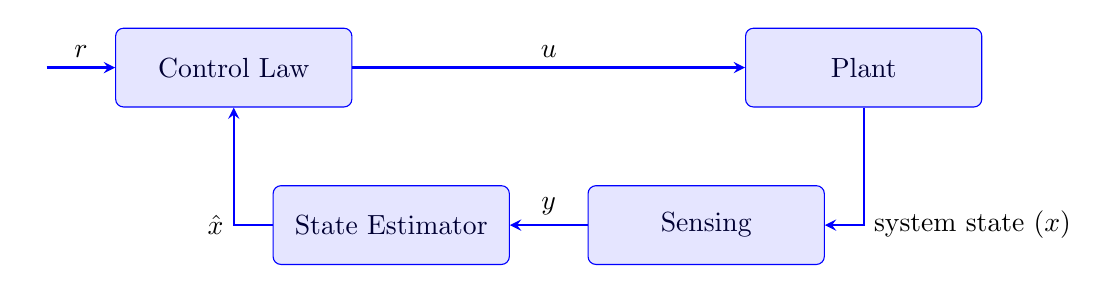
\begin{tikzpicture}[node distance=2cm]
        \node (in) [eNode] {};
        \node (control) [recNodeB, right of=in, xshift=0.5cm] {Control Law};
        \node (sys) [recNodeB, right of=control, xshift=6cm] {Plant};
        \node (sensor) [recNodeB, below of=sys, xshift=-2cm] {Sensing};
        \node (estimator) [recNodeB, below of=control, xshift=2cm] {State Estimator};
        
        \draw [arrowB] (in) -- node[above] { $r$} (control);
        \draw [arrowB] (control) -- node[above] { $u$} (sys);
        \draw [arrowB] (sys) |- node[right] { system state ($x$)} (sensor);
        \draw [arrowB] (sensor) -- node[above] { $y$} (estimator);
        \draw [arrowB] (estimator) -| node[left] { $\hat{x}$} (control);
    \end{tikzpicture}
    
    \caption{A typical feedback control loop where the physical \textit{plant} is monitored via an array of sensors (\textit{Sensing}) which produce noisy sample of the state variables $y$. 
    And after sensing, \textit{State Estimator} aggregates the measurements from all the sensors and produce estimation of the current state $\hat{x}$. Then the \textit{Control Law} produce output to the actuators ($u$) in order to close the gap between the current estimated state and the reference state ($r$).
    \label{fig:control loop}}
\end{figure}

\section{The proposed approach} % (from paper)
\label{sec:architecture}
In this section we elaborate on the specifics of the proposed approach.


\subsection{Architecture}
% TODO: Use the terminology of the figure

In our methodology, we use rich component specification represented by automata.
As presented above, the main advantage of this technique is the ability of the scheduler to ``react'' to the state of the system, therefore we need a richer interaction between the \textit{Scheduler} and the control loops, particularly with the estimator.
The architecture of control system as we believe, is illustrated in Figure~\ref{fig:general_hybrid_loop}.
The architecture, that is based on modern controller architecture where the system has multiple controlling tasks, comes to support an efficient scheduling protocols in modern control systems, consisting of a processor that runs all the tasks of many independent control loops in the system. 
Each control loop (blue components in Figure~\ref{fig:general_hybrid_loop}) will tell the \textit{scheduler} of its level of certainty ($P = var(\hat{x} - x)$) and the scheduler will allocate resource (processor time) based on this data, meaning the \textit{scheduler} allocate resource dynamically based on the system current needs rather than the worst case needs, making the scheduler an active part of the control loop.

%TODO - probably need to be in the Tests section
Our methodology is general and may be applicable in a wide range of applications. However, in this initial phase of the research, we focus on a specific sub-domain and in handling all technical issues in order to prove the concept.
%In this thesis we develop and implement a vision based controller for drone (see Section~\ref{sec:tests}) and analyze the concept with it.

\begin{figure}[h]
    \centering
    
    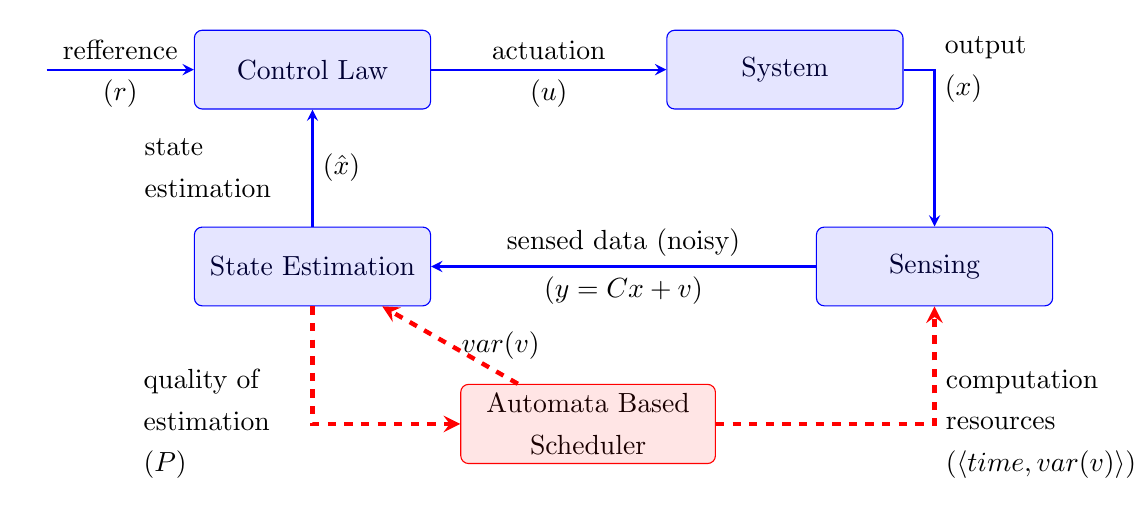
\begin{tikzpicture}[node distance=2cm]
    \node (in) [eNode] {};
    \node (control) [recNodeB, right of=in, xshift=1.5cm] {Control Law};
    \node (sys) [recNodeB, right of=control, xshift=4cm] {System};
    \node (sensor) [recNodeB, below of=sys, xshift=1.9cm, yshift=-0.5cm] {Sensing};
    \node (estimator) [recNodeB, below of=control, yshift=-0.5cm] {State Estimation};
    \node (sched) [recNodeG, below of=estimator, xshift=3.5cm, text width=3cm] {Automata Based Scheduler};
    
    \draw [arrowB] (in) -- node[above] {refference} node[below] {($r$)} (control);
    \draw [arrowB] (control) -- node[above] {actuation} node[below] {($u$)} (sys);
    \draw [arrowB] (sys) -| node[right,text width=1cm] {output ($x$)} (sensor);
    \draw [arrowB] (sensor) -- node[above] {sensed data (noisy)} node[below] {$(y = Cx +v$)} (estimator);
    \draw [arrowB] (estimator) -- node[left,text width=2cm] {state \newline estimation} node[right] {($\hat{x}$)} (control);
    
    \draw [arrowG] (estimator) |- node[left,text width=2cm] {quality of estimation ($P$)} (sched);
    
    \draw [arrowG] (sched) -| node[right,text width=2cm] {computation resources ($\langle time,var(v) \rangle$)} (sensor);
    %\draw [arrowG] (sched) -| node[right] {$\langle time,var(v) \rangle$} (sensor);
    
    \draw [arrowG] (sched) --  node[right] {$var(v)$} (estimator);
    
    \end{tikzpicture}
    
    \caption{The controller framework we implement, Each control loop (depicted in blue) informs the resource allocator (Scheduler) of its quality of estimation, the \textit{scheduler} will allocate CPU time accordingly in order to maintain valid estimation quality. 
        Specifically for the Sensing processes, for example in our case \textit{Computer Vision} task, the guard automaton specify the required sensing quality ($var(v)$) which determines the required execution time ($time$). The Sensing alocation is noted by $\langle time,var(v) \rangle$.
        %The underlying assumption here is that the noise in the sensed data is a function of the amount of computation resources. We assume that the more resources are invested in sensing the better (less noisy) sensed data is obtained.
    \label{fig:general_hybrid_loop}}
\end{figure}

\subsection{Guarded Automata as Interfaces for Control and Scheduling}
As our goal is to allow dynamic selection of the computation load in the feedback loops based on the states of the systems, we start with a general software architecture in which each component (implementation of a specific feedback loop or a sub-task of the controller) is represented by a code module (in our case, a class in C++) and an automaton that specifies when to invoke its methods. The transition relation of the automaton depends, in addition to the current state, also on data produced by the estimator of the feedback loop (we experimented with different options for this data, as discussed below).

The motivations of using automata as described above are: (1) Automata allow for a rich specification language; (2) It is easy to construct schedules that obey the specification with negligible computational burden; (3) Automata theory gives a solid framework for composing the specifications of competing requirements for analysis and for schedule synthesis. 

%TODO - mybe reference to future work section
In this thesis we focus on the first two motivations in the above list. The third is discussed in details in earlier works on automata based scheduling and is the focus of future paper that we are preparing where we describe some analysis techniques we have developed for guarded automata.   

\subsection{Implementation in an Auto Pilot Software}
As our main case study is in flight control (see Section~\ref{sec:caseStudy}), we chose the ArduPilot Mega (APM) platform~\cite{APM} for experiments. To this end, we implemented a basic automata based scheduler for this platform. The built-in task scheduling specification in APM consist of a table as shown in Figure~\ref{fig:apm-scheduler}. This table is easy to maintain and to adjust, but it is used under an assumption that there is enough CPU power to run all the tasks in the specified frequencies. APM does contain a mechanism to handle overruns, by moving tasks to the next window when there is not enough time to run them now, but the system is designed under the assumption that this only happen in rare situations.
%TODO - maybe add APM section in apendex describing this scheduler with image

To allow a reactive scheduler that runs different modes of the software-based controllers depending on their state, we replaced the scheduling table in our version of the APM with automata that specify when to run the tasks. Note that automata allow for specifying the requirements that the table represents, using simple circular automata without guards (see, e.g., \cite{weiss2007automata}). Automata, however, can model more advanced scheduling instructions with very little addition to the complexity of the scheduler, as we will demonstrate in Section~\ref{sec:simulation} and in Section~\ref{sec:caseStudy} below.
%TODO - were gose the detail of the automaton operations

\begin{figure}
    \scriptsize
    \begin{lstlisting}
    /*
    scheduler table - all regular tasks apart from
    the fast_loop() should be listed here, along 
    with how often they should be called (in 10ms 
    units) and the maximum time they are expected 
    to take (in microseconds)
    */
    static const AP_Scheduler::Task 
    scheduler_tasks[] PROGMEM = {
    { update_GPS,            2,     900 },
    { update_nav_mode,       1,     400 },
    { medium_loop,           2,     700 },
    { update_altitude,      10,    1000 },
    { fifty_hz_loop,         2,     950 },
    { run_nav_updates,      10,     800 },
    { slow_loop,            10,     500 },
    { gcs_check_input,       2,     700 },
    { gcs_send_heartbeat,  100,     700 },
    { gcs_data_stream_send,  2,    1500 },
    { gcs_send_deferred,     2,    1200 },
    { compass_accumulate,    2,     700 },
    { barometer_accumulate,  2,     900 },
    { super_slow_loop,     100,    1100 },
    { perf_update,        1000,     500 }
    };
    \end{lstlisting}
    \caption{APM scheduling specification}
    \label{fig:apm-scheduler} 
\end{figure}

\subsection{Integration With a Kalman Filter}
\label{sec:Arch-kalman}
The third layer of the approach we propose is based on the observation that a standard Kalman filter produces information that can be used to guide the automata of the components. 

As we will elaborate in the description of the simulations and of the case study below, we propose to schedule the functions that implement algorithms for sensing and for actuation based on the estimation quality as reported the Kalman filter (denoted by $P$ in Figure~\ref{fig:general_hybrid_loop}).
The estimation quality ($P$) is passed to the scheduler, then the scheduler schedules higher quality sensing if $P$ is less than the required value and lower quality sensing otherwise. Then, of course, the scheduler reports the current sensing quality to the Kalman filter (denoted by $var(v)$ in Figure~\ref{fig:general_hybrid_loop}).   
This way, we schedule different sensing modes in order to \textbf{adjust} the quality of estimation ($P$).
There are two basic values that we can use for the quality of estimation ($P$):

The first option is to use directly the estimate covariance ($P_{k|k}$) that the Kalman filter produces (see Section~\ref{sec:kalman}). This technique can be used if we just need to adjust or control the error covariance of the estimation. This is offline scheduling, as the value of $P_{k|k}$ is not affected by the environment, i.e., it is calculates only by the noise covariance, not the measured data.
    
The second option is the technique we implement in this thesis (Section~\ref{sec:Analysis}) is trying to estimate the overall noise of the system, actuating, sensing and process noise together. Here, instead of using $P_{k|k}$, we use the quality measure $\tilde{y}_{k|k}$ which represents the difference between the expected measurement (in case that all the noises are zero) and the actual measurement that was observed. By this definition $\tilde{y}_{k|k}$ is an approximation of the overall noises.
    
We call this technique `adaptive scheduling' or `reactive scheduling'. We show in this thesis that it is powerful in cases where the system behavior is not monotonic, e.g., when we may observe different light sources with vision sensing or changing battery states, or in cases that the system behavior is not precisely known.


\section{A demonstration of the approach in simulation}
\label{sec:simulation}
%TODO - explain that we developing an idea that culd in the future become a tool

Our approach for using automata for scheduling resources in software based controllers, is based on the observation that in most systems the computational load is in the implementation of the sensors and actuators, not in the implementation of the controllers that usually consist of quick arithmetic manipulation of a small amount of variables. We therefore focus our attention on allowing a trade-off between CPU usage of sensors and actuators and their accuracy. %In this work, as a main motivating example, we focus on the case of visual sensors that employ image processing algorithms.

As said in Section~\ref{sec:architecture}, we propose to implement the resource scheduling decisions using automata that control which procedures are invoked in the control loops. More specifically, for sensors or actuators that require heavy computations, such as vision based sensors, we propose that the software engineers develop several modes of sensing, each consumes a different amount of CPU and provides a different level of accuracy. 
%In Figure~\ref{fig:simulink} there is an example of a controlled system, in this case an open control loop, that its state is observed using multi-level vision based sensors 

Formally, we assume that each of the physical processes we control are a Linear Time Invariant (LTI) system with a known model, as depicted in Figure~\ref{fig:simulink}. 
The figure shows a controlled system, in this case an open control loop, that its state is monitored via vision based sensor. 
The inaccuracies of the sensors and of the actuators are modeled as additive Gaussian noise with a known variance. As a basis for scheduling, we assume that each sensor (and, possibly, also the actuators) can be scheduled to operate in one of a range of modes at each computation slot, each mode consuming a certain percentage of the CPU and giving a certain variance of the measurement (or actuation) noise.

\begin{figure}%[htbp]
    \centerline{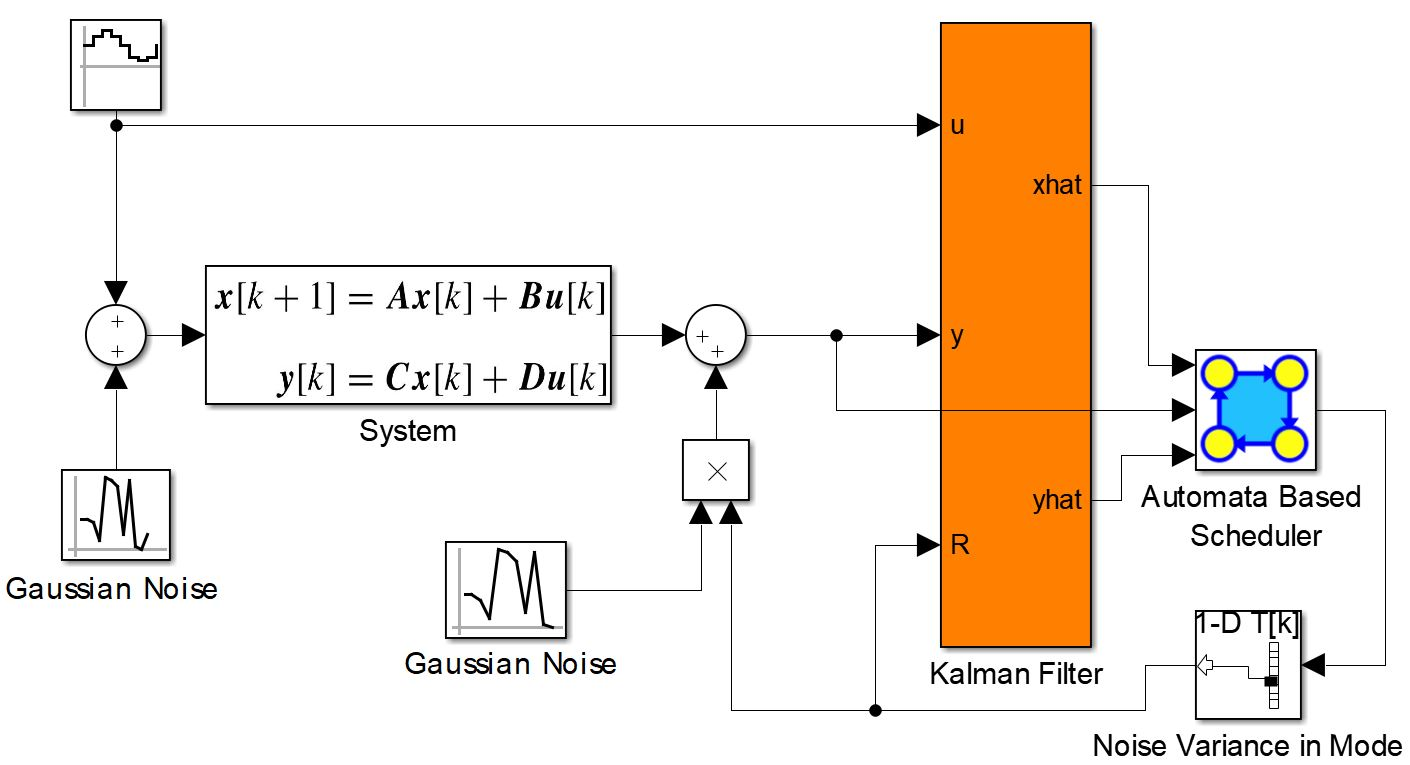
\includegraphics[width=100mm]{SimulinkModel.jpg}}
    \caption{A Simulink model used to demonstrating and  examine the proposed approach.}
    \label{fig:simulink}
\end{figure}

The scheduling of the modes, for each of the components, is governed by the automata based scheduler as depicted in Figure~\ref{fig:simulink}. We propose to use a standard Kalman filter as a tool to gather the information that guides the state evolution of the automata, as follows. The filter gets as input the actuations ($u$),  measurements ($y$), and the covariance matrix of the measurement noise ($R$). We assume that the measurement noise is a static function (represented here as a translation table) of the mode chosen by the scheduler. The output of the Kalman filter is fed to the scheduler that uses it for advancing the states of the automata. 
In the Simulink model depicted in Figure~\ref{fig:simulink}, the covariance matrix of the disturbance, which in this case is $1 \times 1$ matrix consisting of the noise variance, is fed to the Kalman filter (as its $R$ input) and to the block that multiplies the Gaussian noise by the variance (the product of a white noise with unit variance and a constant $v$ yields a Gaussian noise with variance $v$).

We ran the model depicted in Figure~\ref{fig:simulink} with the linear time invariant system
\begin{eqnarray*}
    x(k+1) &=& \begin{pmatrix}        1.3  & -0.5  & 0.1 \\
        1    & 0     & 0 \\
        0    & 1     & 0
    \end{pmatrix}x(k)+ 
    \begin{pmatrix}
        -0.4 \\
        0.6\\
        0.5\end{pmatrix} u(k) \\
    y(k)&=& \begin{pmatrix}1 & 0 &0\end{pmatrix}x(k)
\end{eqnarray*}
taken from \url{mathworks.com/help/control/examples/kalman-filter-design.html}. As seen in Figure~\ref{fig:simulink}, we injected a sinusoidal input (with $amplitude=bias=frequency=1$) to this system. 
The actuation noise, depicted on the left, is with a unit variance. 

The `Automata Based Scheduler' block is designed to set the variance of the sensing noise dynamically to be either $0.25$ or $1$ at each step of the simulation. This models a sensor that has two modes of operation: a mode with high accuracy, that produces normally distributed measurement errors with low variance, and a mode with low accuracy that produces normally distributed measurement errors with higher variance. We assume, for the performance measurements presented below, that the CPU consumption of each mode is $\%CPU=1.1-errVar$, where $errVar$ is the variance of measurement errors in the mode.

We ran this model with three versions of the `Automata Based Scheduler' block. The first version, called `High' in Table~\ref{tbl:sim-results}, is where the block acts simply as the constant $1$, ignoring its inputs altogether. Similarly, the term `Low' in the table refers to an implementation where the block is the constant $0$. These two implementations model the constant schedules, where the sensor is operated in one mode along the whole execution. These two schedules are compared to a third implementation, called 'Aut. Based' in the table, where the block implements the schedule given by the automaton:
\begin{center}
    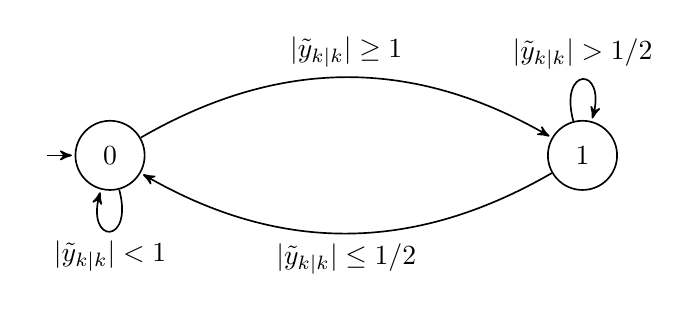
\begin{tikzpicture}[->,>=stealth',shorten >=1pt,auto,node distance=6cm,
    semithick]
    
    \node[initial,state] (A)                 {$0$};
    \node[state]         (B) [right of=A]    {$1$};
    
    \path (A) edge [bend left]             node {$|\tilde{y}_{k|k}|\geq1$} (B)
    (A) edge [loop below] node {$|\tilde{y}_{k|k}|<1$} (A);
    
    \path (B) edge [bend left]             node {$|\tilde{y}_{k|k}|\leq 1/2$} (A)
    (B) edge [loop above] node {$|\tilde{y}_{k|k}|>1/2$} (B);
    
    \end{tikzpicture}
\end{center}
The states of the automaton represent operation mode of the sensor, 0 for `Low' mode and 1 for `High' mode.
$|\tilde{y}_{k|k}|$ which equals to $|y-\hat{y}|$ means how far is the last measurement from the expected measurement this value, and act as indication of the overall real noises, process, measurement and actuation noises together, as elaborated in Section~\ref{sec:Arch-kalman}.
The automaton try to formalize the expression: ``use `High' mode only after observing high distributed''.

%A = [1.1269   -0.4940    0.1129,
%1.0000         0         0,
%0    1.0000         0];
%
%B = [-0.3832
%0.5919
%0.5191];
%
%C = [1 0 0];

\begin{table}
    \centering
    \begin{tabular}{ |  l  | c | c | c | }
        \hline
        &  High & Low & Aut. Based \\ \hline \hline
        \%CPU                    & 85 & 10  & 46 \\ \hline
        mean of $|x -\hat{x}|$ & 0.97 & 1.24 & 1.08 \\ \hline
    \end{tabular}
    \caption{Simulation results.}
    \label{tbl:sim-results}
\end{table}

The results of the simulation, summarized in Table~\ref{tbl:sim-results}, show, as expected, that the CPU consumption is much lower (0.1) when using the low-quality version of the sensing algorithm and is higher (0.85) when the high-quality version of the sensing algorithm is used. The performance of the estimation, in terms of the mean distance between $x$ (the real state) and $\hat x$ (the Kalman filter estimated state), is better with the high-quality version (0.97) than it is with the low-quality version (1.24). More interestingly, we can see that the experiment with the automaton that switches between the two sensor modes yields performance that is close to the performance of the high-quality sensing algorithm, using much less CPU. This demonstrates how automata based reactive scheduling can allow for new ways to balance performance and computational resources in software based controllers. 

\section{Case Study: Stabilizing a Quad-rotor in Front of a Window}
\label{sec:caseStudy}
% overview of why we use vision example

The case study we used to test our concept is the development of a controller that stabilizes a quadrotor in front of a window (see, e.g.,~\url{rpg.ifi.uzh.ch/aggressive_flight.html}).
We implemented an autonomous controller for that task and evaluated its performance.

The part of the controller that we focused on is the vision based position controller. Specifically, the main controller, that we will describe below, uses a standard low-level angular controller and a simple image processing algorithm that identifies the position of the corners of the window in the image plane\footnote{In the experiment, to simplify the image processing algorithm, we marked the corners of the window with led lights.}. Its goal is to regulate the position of the quadrotor by tilting it. Note that rotations of the quadrotor by a small angle generate a more-or-less proportional accelerations in a corresponding direction, hence we can approximate the system with a linear model. A main challenge for this controller is that the computer vision algorithm takes significant time to compute relative to the fast control loop. We can decrease computation time by lowering the resolution, but this also increases the measurement noise. We will demonstrate how reactive scheduling of the resolution can serve for balancing resource consumption vs. control performance in this system.

\subsection{Observer Design}
\label{sec:Observer Design}
We first implemented an observer based on the work of Efraim~\cite{Efraim17}. The observer gets the positions of the widow corners from the image (see Section~\ref{sec:Experiment setup-cam} for more details), %enumerated clockwise starting from the top left corner noted by $p_1,p_2,p_3,p_4$, 
and extracts the following four quantities based on the shape and location of the window corners in the image plane: %$S_x$, $S_y$, $V_d$ and $sz$, as follows.
\textbf{Center of mass:} $S_x$ and $S_y$ represent the window ``center of mass'' along the $x$ and $y$ axes of the image, respectively, normalized to the range of $[-1,1]$.
These values are used for controlling the yaw angle and the altitude of the drone, respectively. The controller tries to drive these variables to zero so that the drone will  always face the center of the window and hover at the altitude of the center of the window. 
\textbf{Window size:} $sz$ is the sum of the vertical edges of the window. It is used to measure the distance of the drone from the window~\footnote{We used a fixed size window and converted $sz$ to distance (in meters in our case) based on the size of the window. In the general case the units of distance are relative to the window size.}.
\textbf{Vertical difference:} $V_d = {((y_1-y_4)-(y_2-y_3))}/{((y_1-y_4)+(y_2-y_3))}$, where $y_i$ is the vertical position of the widow corners in the image in the range of $[-1,1]$, enumerated clockwise starting from the top left corner. It is measure the angular position of the drone in relation to the window (parallel to the ground) and used to control the position of the drone among the $x$ axis.
Note that although $V_d$ does not directly measure the linear $x$ position of the drone, we can estimate the linear $x$ position by simple geometry:
as shown in Figure~\ref{fig:V_d-geomerty} $x = l \cdot \sin (V_d)$ where $l$ (distance from window) can be calculated from $sz$. In our case because $V_d$ is usually relatively small we approximate it by $x = l \cdot V_d$.

\begin{figure} %[htbp]
    \centerline{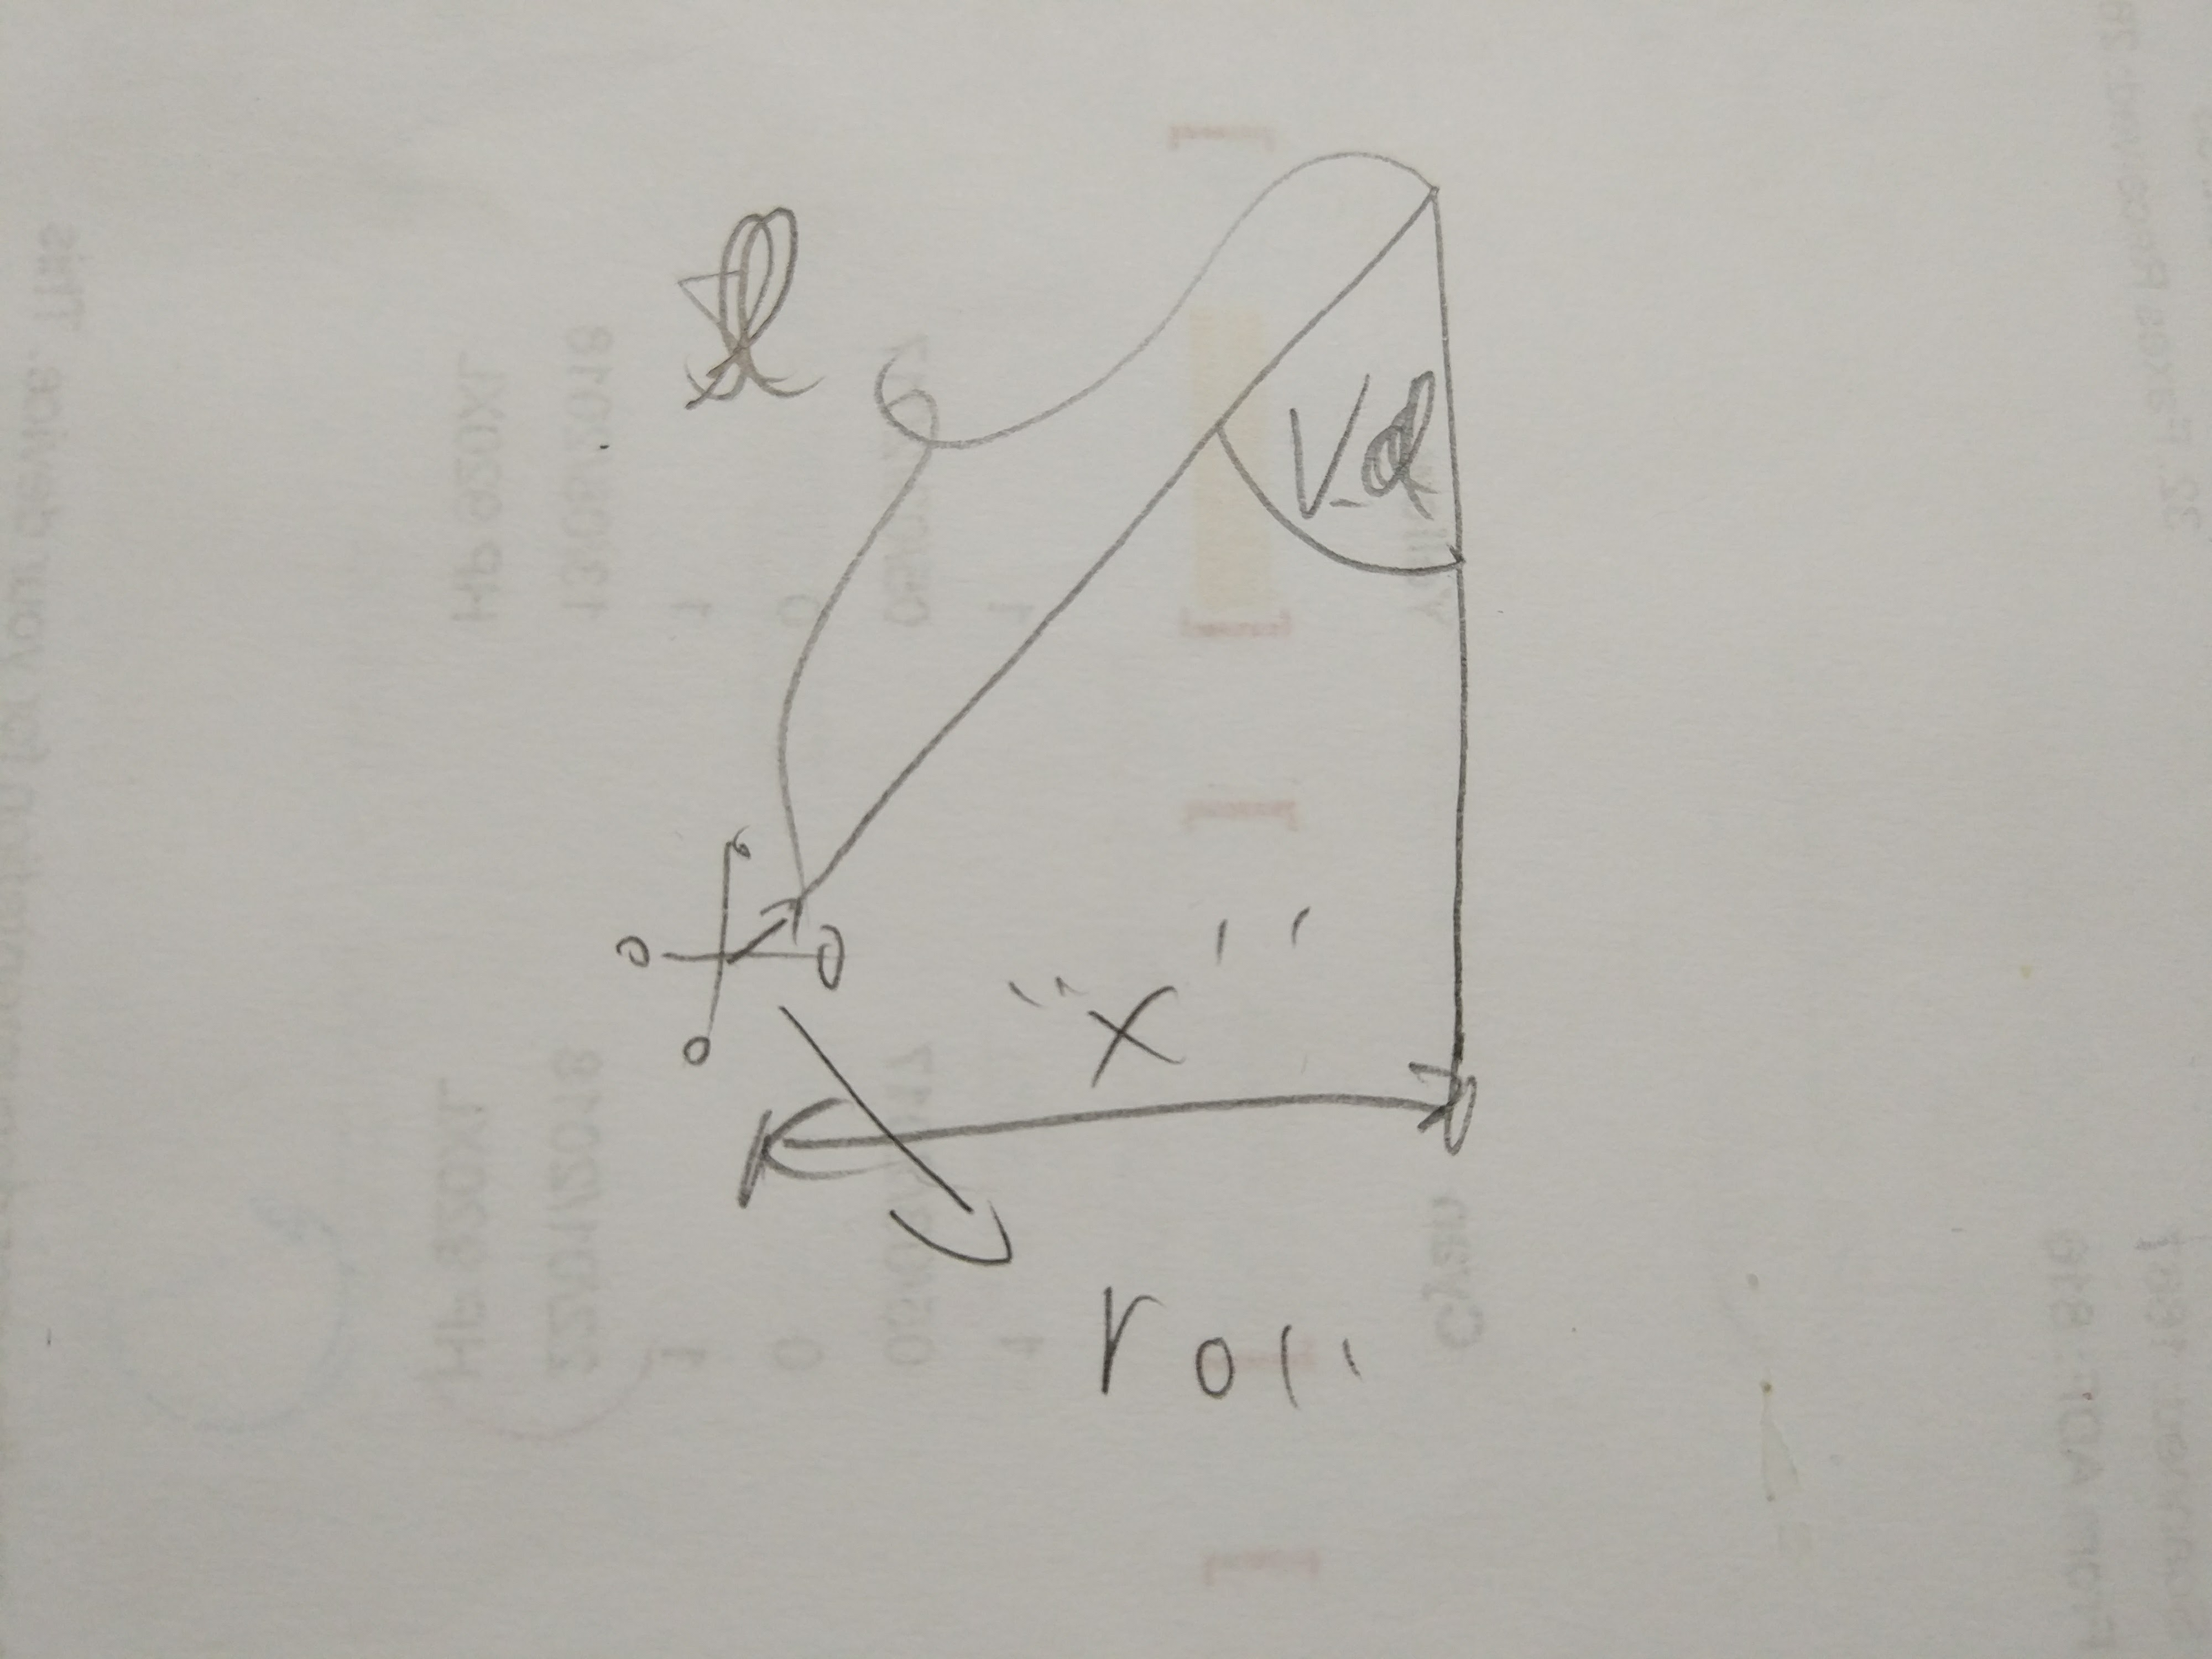
\includegraphics[width=80mm]{vd-geometry.jpg}}
    \caption{Geometric relation between $\alpha$ (the angle derived from $V_d$) $l$ (distance from window extracted from $sz$) and the position of the drone among the $x$ axis.}
    \label{fig:V_d-geomerty}
\end{figure}


As common in engineering practices, we pass these numbers to a filter that gives us a state estimation. 
Ideally, when the system is linear as in the simulations in Section~\ref{sec:simulation}, we should use a Kalman filter for best state estimation. As we deal with a non-linear system here, and because the process noise distribution is not known (it is significantly affected by the varying state of the battery), and because a Kalman filter adds complexity in the code, we use a complementary filter.
Complementary filters can implement the steady-state (when the Kalman gains converge) behavior of Kalman filters~\cite{complementaryVSKalman}.
Specifically, in our case study, we implemented a two steps estimator that: (1) \textit{predicts} the current state evolved from the previous state, denoted by $\hat{x}_{k|k-1}$, using a linearized model of the system, and then \textit{updates} the prediction with current state measurement from the image, denoted by $y_k$.
The result of the estimation, denoted by $\hat{x}_{k|k}$, is a complementary filter of the prediction ($\hat{x}_{k|k-1}$) and the measured state ($C^{-1}y_k$)~\footnote{The matrix $C$ is the measurement matrix as shown in the model at Figure~\ref{fig:simulink}. For simplicity, the text is under the assumption that $C$ is not not singular. If $C$ is singular, one can use the observability matrix in a similar fashion, assuming that the system is observable.}:
$ \hat{x}_{k|k} = K \hat{x}_{k|k-1} + (1-K) C^{-1}y_k $ were $K$ is a constant that approximates the Kalman filter gain ($K_k$) at a steady-state, see Section~\ref{sec:kalman} for more details.
The constant $K$ represents the ratio between the variance of the process noise and the variance of the measurement noise. To achieve best performance, we define a different value of $K$ for each mode corresponding with the image resolution and the noise variance.

\todo[inline]{need to add section on the system linearized model? maybe the Figure~\ref{fig:acceleration_static_diagram} is enough}



\begin{figure} %[htbp]
    \centerline{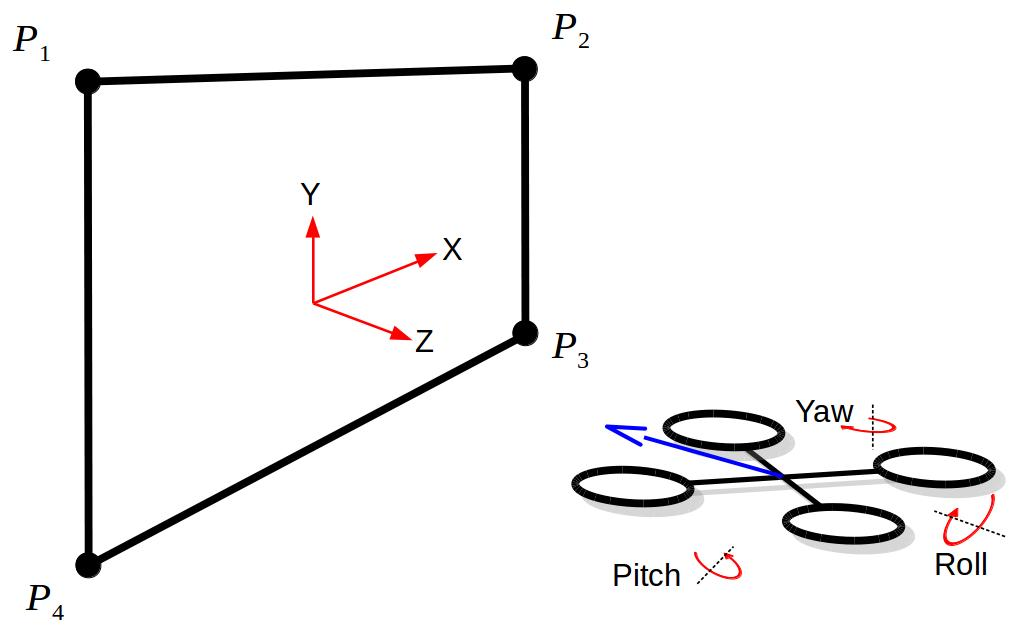
\includegraphics[width=100mm]{axis.jpg}}
    \caption{The coordinate system and the rotation axes of the drone, the position axis ($x$, $y$ and $z$) are in relation to the window, ``yaw'' angle is the horizontal angle of the center of the window related to the front of the drone, ``pitch'' and ``roll'' are angles of the drone itself (calculated from the inertial sensors only).}
    \label{fig:axis}
\end{figure}

\subsection{Controller Design}
\label{sec:Controller Design}

In this experiment, we consider the task of hovering in front of the window. The controller objective is to hover parallel to the window (center of $z$ axis in Figure~\ref{fig:axis}) at the altitude of the window within distance of two meters in front of the window ($y=x=0 , z=2$) and face to the center of the window (yaw angle).
We consider this point as the desired position and use the coordinate system depicted in Figure~\ref{fig:axis}.

The controller consists of four independent feedback loops: altitude, yaw, pitch, and roll.
The pitch and the roll controllers are copies of the same attitude controller which gets as input the required pitch or roll angel, respectively. These controllers runs in parallel to a position controller that maintains the required distance ($z$ position) and displacement ($x$ position) relative to the window. The position level controller outputs the required angle (acceleration) to the attitude controller as show in Figure~\ref{fig:controllerStracture}.
Altitude, yaw, $x$, and $z$ position are regulated relative to the window.
The inertial pitch and roll feedback for the low level controllers is related to the drone body and is generated by the existing \textit{Attitude and Heading Reference system} (AHRS) library of ArduPilot (see Section~\ref{sec:Experiment setup}) and the position feedback ($x$, $y$, and $z$ position) comes from the observer described in Section~\ref{sec:Observer Design}.

\begin{figure} %[htbp]
    \centerline{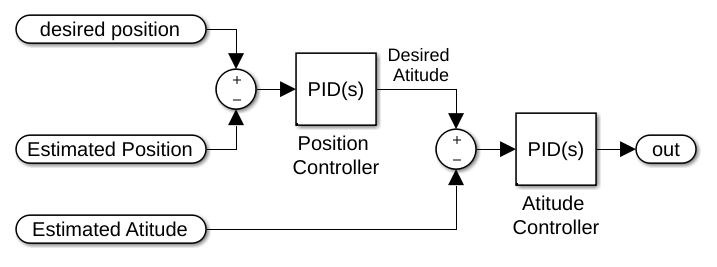
\includegraphics[width=100mm]{two_level_controller.jpg}}
    \caption{Attitude and position controller consisting of a two level, cascaded, structure.}
    \label{fig:controllerStracture}
\end{figure}

%TODO - some conversion proof
The position controller is as follows:
The altitude ($y$ position) is obtained directly from the $S_y$ value explained in Section~\ref{sec:Observer Design} and it is regulated by changing the overall ``throttle'' of the rotors, this approach works well assuming that the drone pitch and roll angles are close to zero. In this case, $S_y$ is almost proportional to the real altitude of the drone and the trust vector is pointed up.
The $z$ position is assumed to be the distance from the center of the window, which we assume is proportional to the window size ($sz$). It is regulated by changing the pitch angle. Assuming the drone is always facing the center of the window (yaw angle is zero) the pitch angle produces acceleration in the pitch direction, i.e., it can be use to regulate $z$.
The $x$ position (displacement) is regulated by changing the roll angle. Similar to $z$ position, assuming the drone is always facing the center of the window, the roll angle produces acceleration that increase or decrease the $x$ position depending on the roll angle direction.

As demonstrated in Figure~\ref{fig:acceleration_static_diagram}, the acceleration in the $x$ direction is $a_x=g \arctan(\alpha_{roll})$ and the acceleration in the $z$ direction is equal to $a_z=g \arctan(\alpha_{pitch})$. 
In practice, in this work we usually assume a linearized proportional acceleration model, i.e., $a_x=g \cdot \alpha_{roll}$ and $a_z=g \cdot \alpha_{pitch}$.

Note that if $x$ is not zero the drone is not parallel to the window and the roll direction (that used to regulate $x$ position) also affects the $z$ position.
Similarly, if the drone is not parallel to the window and the pitch direction (that used to regulate $z$ position) also affects the $x$ position.
Although in theory $x$ controller disturb the $z$ controller and vice versa, in practice even if the drone displacement is relatively large, when all the controllers are executed together (and are tuner correctly) they constantly fix those side-afects and because the $x$ position is generally decreased during this process we eventually converge to a stable state were the drone is near-parallel to the window.

\begin{figure} %[htbp]
    \centerline{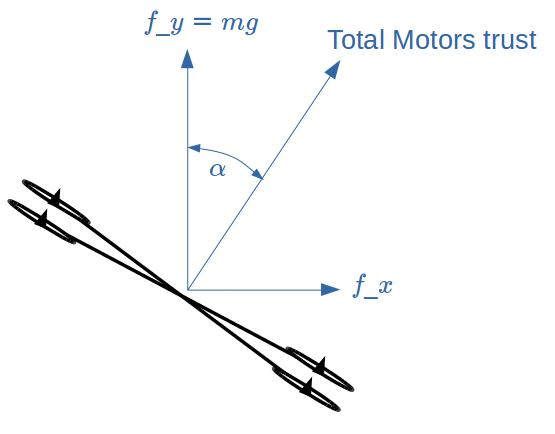
\includegraphics[width=80mm]{acceleration_static_diagram.jpg}}
    \caption{Free body diagram (force diagram) of the drone $x-y$ or $z-y$ plane forces, this diagram demonstrates the relation between $x$ or $z$ acceleration ($a_x$ or $a_z$) and the corresponding tilt angle. $\alpha$ represents the tilt angle (roll or pitch) and $a$ represents the acceleration in the corresponding direction. We assume that the altitude controller works as expected and the vertical speed is close to zero ($a_y = 0$), and we get $m a = \arctan(\alpha) \cdot mg$, that is, the acceleration is $a = \arctan(\alpha) \cdot g$ we use tis relation for the controller design (Section~\ref{sec:Controller Design}) and we also use this calculation as part of the system model in the Observer (see Section~\ref{sec:Observer Design}). }
    \label{fig:acceleration_static_diagram}
\end{figure}

Based on the \textit{principle of separation of estimation and control}~\cite{aastrom2012introduction}, we can use that controller regardless of the measurement quality. Therefore, we implemented a basic Proportional Integral Derivative (PID~\cite{aastrom2006advanced}) controller and tuned the parameters by trial and error using the highest resolution observer.

%%%%%%%%%%% Specification Automata %%%%%%%%%%%%%
\subsection{Analysis and Specification Automata}
\label{sec:Analysis}

The objective of the system is to maintain stable hovering in front of the window, for analysis, performances is measured by the amount of deviation from the center line of the window in the $x$ axis, i.e., we want to minimize $\left| x \right|$ (see Figure~\ref{fig:axis}).
Our goal is to achieve maximum performance with minimal amount of processing time.
Obviously, both goals cannot be achieved together. We therefor aim at achieving a good and flexible trade-off between processing resources and quality of measurement. The focus is on the main consumer of computation resources: the image processing algorithm.
We aim at taking resources (high CPU time) only when needed. By this, we will reduce the average CPU usage without significantly affecting the performance.
Specifically in our case study, we switch between camera resolutions dynamically during the flight. The observer modes, discussed above, correspond to image resolutions (see Section~\ref{sec:Observer Design}).
For simplicity, we consider in this thesis only two modes: \textit{High quality} with resolution of 960p and \textit{Low quality} with resolution of 240p.

Looking at the test results shown in Table~\ref{tab:results}, we see that the high quality observation mode provides mean error tolerance of 9.5\textit{cm} (in the $x$ axis) with the cost of 30\% CPU usage.
On the other hand, the low quality mode provides mean error of 30\textit{cm} (three times the error obtained in the high quality mode) using only 2.1\% CPU usage~\footnote{The CPU usage percentage is the average: (total time spend in image processing)/(total flight time). }.

We explain next several approaches we applied in the design of a \textit{reactive scheduling specification} that combines both, high and the low resolution sensing modes in an sufficient way.

%displacement ($x_{k|k}$) schedulers
We first examined a straight-forward scheduler based directly on the current position (the $x$ axis value). Using the simple guarded automaton $A_{x}$ presented in Figure~\ref{fig:test_automata}, we defined a dynamic observer that chooses the mode (high or low sensing quality) based on the current absolute value of the $x$ axis ($x$ coordinate of $\hat{x}_{k|k}$). If the drone is closer to the center line of the window, denoted by $|x| < T_x$, we consider it as a ``safe'' state and go to the mode called $L$ that schedules the low quality image.
Similarly, a state is considered ``BAD'' when the drone is far, denoted by $|x| > T_x$. In this case, we take high quality images in order to ``fix'' the state.
The threshold $T_x$ can be changed to tune the desired performances and processing time trade-off.
See Section~\ref{sec:results} for the data we collected by experiments to validate that this indeed achieves the required goals. 
% Results shows good improvement in term of resource utilization (see Section~\ref{sec:results}). 

%error ($y_{k|k}$) schedulers
In a second experiments set, we used the $A_{err}$ automaton presented in Figure~\ref{fig:test_automata}. This automaton is similar to $A_x$ with the difference that it switches states based on the \textit{measurement post-fit residual} $\tilde{y}_{k|k}$ value, as presented in Section~\ref{sec:Arch-kalman}, and defined as:
$$\tilde{y}_{k|k} =  C\hat{x}_{k|k} - y_k $$
Where $C\hat{x}_{k|k}$ is the expected measurement and $y_k$ is the real measurement at time $k$.

The motivation to use this indicator comes form looking at the low quality experiment graph, shown in Figure~\ref{fig:testPlot}. We can see that $\left| \tilde{y}_{k|k} \right|$ growth is proportional to the deviation from the center of the window (in the $x$ axis). 
%We can also see that the growth in $\left| \tilde{y}_{k|k} \right|$ precedes the growth in $x$. 
This means that we can use $\left| \tilde{y}_{k|k} \right|$ values to predict deviations in $x$.

In $A_{err}$ the observer operates in low quality when $\left| \tilde{y}_{k|k} \right| < T_{l}$ (``GOOD'' state) and switches to high quality when $\left| \tilde{y}_{k|k} \right| > T_{h}$ (``BAD'' state).
The thresholds $T_{l}$ and $T_{h}$ were initially taken from the low and the high quality graphs and fine tuned by experiments. 
Different $T_{l}$ and $T_{h}$ give different trade-offs of performances and processing time.
In Section~\ref{sec:results} we show that this dynamic observer gives almost the same performance as the high quality observer with a reduction of a factor of two in the processing load.

%complex / agregated schedulers (3-4 states)
The expressiveness of automata allows for creating even more complex scheduling specification. We can, for example, combine the approaches of both $A_{err}$ and $A_{x}$.
In Figure~\ref{fig:test_automata} there is two examples of such combinations. $A_{comp1}$ tries to save unnecessary CPU usage while the drone is in ``safe'' state, close to the center. It activates $A_{err}$ only if the drone goes far from the center ($T_{x}$cm from the origin).
$A_{comp2}$ adds another constraint: if the drone goes even farther away ($T_{x2}$cm from the origin) it schedules only high resolution to bring it back to safety.
The results show even better resource utilization.

\begin{figure} %[htbp]
    \centerline{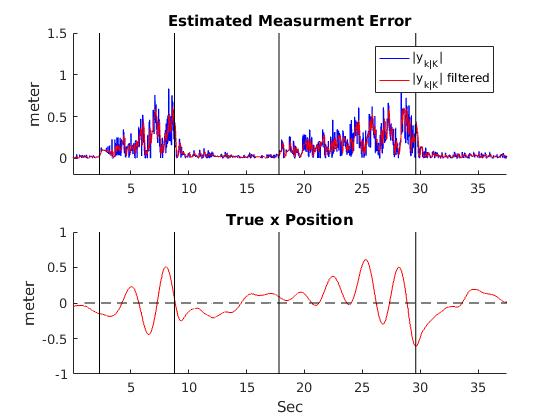
\includegraphics[width=100mm]{errorVsPosition.jpg}}
    \caption{This figure shows in the bottom plot the position of the quadrotor during the flight time and in the top plot the $\left| \tilde{y}_{k|k} \right|$ value during the flight. During the flight we manually switched between low and high resolution for further analysis. The modes (high or low) are separated by vertical lines, were the leftmost is high resolution then low and so on.}
    \label{fig:testPlot}
\end{figure}


%%%%%%%%%%%%%%%%%%%%%%%%%%%%%%%%%%%%%%%%%%%%%%%%%%
%%%%%%%%%%%%%%% automata %%%%%%%%%%%%%%%%%%%%%%%%%
%%%%%%%%%%%%%%%%%%%%%%%%%%%%%%%%%%%%%%%%%%%%%%%%%%
\tikzset{every edge/.append style={font=\small}}
\tikzset{every node/.append style={font=\small}}
\begin{figure} %[htbp]
    %\captionsetup{width=0.4\textwidth}
    \centering
    \begin{tabular}{c c}
        % by error
        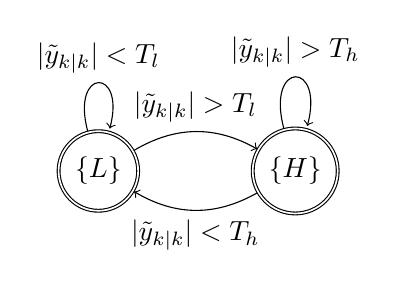
\begin{tikzpicture}[node distance=2.5cm,auto]
        \node (A) [state, accepting] {$\{L\}$};
        \node (B) [state, accepting] [right of=A] {$\{H\}$};
        
        \path[->] (A) edge [loop above] node {$|\tilde{y}_{k|k}| < T_l$} (A);
        \path[->] (A) edge [bend left] node {$|\tilde{y}_{k|k}| > T_l$} (B);
        \path[->] (B) edge [bend left] node {$|\tilde{y}_{k|k}| < T_h$} (A);
        \path[->] (B) edge [loop above] node {$|\tilde{y}_{k|k}| > T_h$} (B);
        %\path[->] (B) edge [bend left] node {$s_{0.7} \wedge est_1$} (A);
        \end{tikzpicture}
        
        &
        
        % by displacement (|x|)
        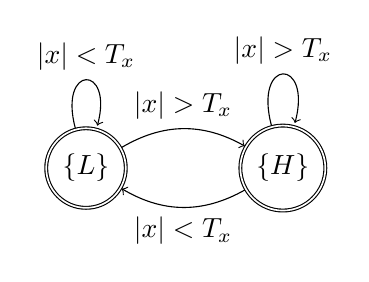
\begin{tikzpicture}[node distance=2.5cm,auto]
        \node (A) [state, accepting] {$\{L\}$};
        \node (B) [state, accepting] [right of=A] {$\{H\}$};
        
        \path[->] (A) edge [loop above] node {$|x| < T_x$} (A);
        \path[->] (A) edge [bend left] node {$|x| > T_x$} (B);
        \path[->] (B) edge [bend left] node {$|x| < T_x$} (A);
        \path[->] (B) edge [loop above] node {$|x| > T_x$} (B);
        %\path[->] (B) edge [bend left] node {$s_{0.7} \wedge est_1$} (A);
        \end{tikzpicture}
        
        \\
        \LARGE{$A_{err}$} & \LARGE $A_x$ \\[10pt]
        \hline
        
        % 3 state
        \multicolumn{2}{c}{
            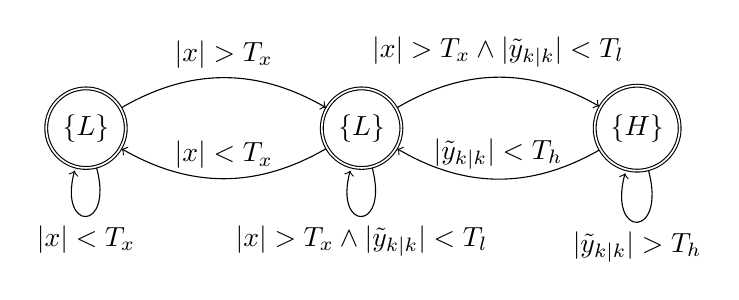
\begin{tikzpicture}[node distance=3.5cm,auto]
            \node (A) [state, accepting] {$\{L\}$};
            \node (B) [state, accepting] [right of=A] {$\{L\}$};
            \node (C) [state, accepting] [right of=B] {$\{H\}$};
            
            \path[->] (A) edge [loop below] node {$|x| < T_x$} (A);
            \path[->] (A) edge [bend left] node {$|x| > T_x$} (B);
            \path[->] (B) edge [bend left, above] node {$|x| < T_x$} (A);
            \path[->] (B) edge [loop below] node {$|x| > T_x \wedge |\tilde{y}_{k|k}| < T_l$} (B);
            
            \path[->] (B) edge [bend left] node {$|x| > T_x \wedge |\tilde{y}_{k|k}| < T_l$} (C);
            \path[->] (C) edge [bend left, above] node {$ |\tilde{y}_{k|k}| < T_h$} (B);
            \path[->] (C) edge [loop below] node {$ |\tilde{y}_{k|k}| > T_h$} (C);
            %\path[->] (B) edge [bend left] node {$s_{0.7} \wedge est_1$} (A);
            \end{tikzpicture}
        }
        
        \\ 
        \multicolumn{2}{c}{\LARGE $A_{comp1}$}\\[10pt]
        \hline
        
        % 4 state
        %TODO - Hodai say: this is non-deterministic automata for sipmlicity
        \multicolumn{2}{c}{
            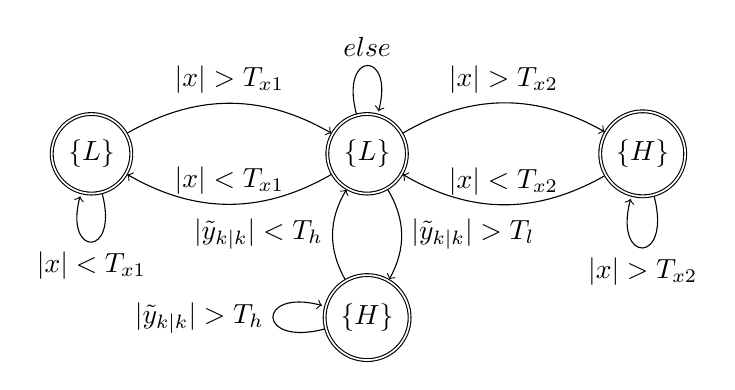
\begin{tikzpicture}[node distance=3.5cm,auto]
            \node (A) [state, accepting] {$\{L\}$};
            \node (B) [state, accepting] [right of=A] {$\{L\}$};
            \node (C) [state, accepting] [right of=B] {$\{H\}$};
            \node (D) [state, accepting] [below=1cm of B] {$\{H\}$};
            
            \path[->] (A) edge [loop below] node {$|x| < T_{x1}$} (A);
            \path[->] (A) edge [bend left] node {$|x| > T_{x1}$} (B);
            \path[->] (B) edge [bend left, above] node {$|x| < T_{x1}$} (A);
            
            \path[->] (B) edge [loop above] node {$else$} (B);
            
            \path[->] (B) edge [bend left] node {$|x| > T_{x2}$} (C);
            \path[->] (C) edge [bend left, above] node {$|x| < T_{x2}$} (B);
            \path[->] (C) edge [loop below] node {$|x| > T_{x2}$} (C);
            
            \path[->] (B) edge [bend left] node {$|\tilde{y}_{k|k}| > T_l$} (D);
            \path[->] (D) edge [bend left] node {$|\tilde{y}_{k|k}| < T_h$} (B);
            \path[->] (D) edge [loop left] node {$|\tilde{y}_{k|k}| > T_h$} (D);
            \end{tikzpicture}
        }
        \\
        \multicolumn{2}{c}{\LARGE $A_{comp2}$}\\
        
        
    \end{tabular}
    
    \caption{The main Automata we used for the requirements specifications in the experiments. 
        $A_{err}$ uses the \textit{measurement post-fit residual} ($\tilde{y}_{k|k}$), if $|\tilde{y}_{k|k}|$ is too small then the next iteration will use small resolution image ($L$), and if it is too large the high resolution will be used, $T_l$ and $T_h$ are the transition thresholds.
        $A_x$ operates similar to $A_{err}$, only it uses the current position (the $x$ part of $\hat{x}_{k|k}$) instead of $\tilde{y}_{k|k}$, with the threshold $T_x$.
        $A_{comp1}$ and $A_{comp2}$ area composition of the ideas in $A_{err}$ and in $A_x$.}
    
    \label{fig:test_automata}
\end{figure}

%%%%%%%%%%% results %%%%%%%%%%%%%
\section{Results}
\label{sec:results}

Table~\ref{tab:results} summarizes the result of the flight experiments made using the specification automata described in Section~\ref{sec:Analysis}.
The first column ``\% CPU'' represents processing time usage by the image processing task.
The second column ``$mean(|$x$|)$'' is the average distance of the drone from the origin in centimeters.
All the statistics shown in the table are from real indoor experiment flights. Each experiment consists of a flight (between one and two minutes) recorded with the \textit{OptiTrack} system (see Section~\ref{sec:Experiment setup-optitrack}) and with data from the software itself.

We see that, using reactive scheduling methods, we can adjust the trade-off between performance and CPU usage. As expected, if we use \textbf{only high} resolution mode we get the best performance but need much \%CPU. On the other hand, the \textbf{only low} resolution mode barely use the processor but the performance are low and unsatisfying for indoor flights.

In Table~\ref{tab:results}, automata number 3,4 and 5 are the implementation of $A_{x}$ automaton as describe in Section~\ref{sec:Analysis} with the threshold values of 10, 20 and 30cm respectively.
Those schedulers demonstrate that even a simple scheduling scheme, that schedules the expensive image processing task only when the state is critical, improves the performance. Scheduler number 3 achieves almost the same performance as the only high resolution scheduler but saves half of the CPU time. Scheduler automata 4 and 5 provide different trade-offs.

The $A_{err}$ automaton (shown in Figure~\ref{fig:test_automata}), which bases its transitions on $\tilde{y}_{k|k}$, appears to be even more effective.
We tested this automaton with ($T_l=10 , T_h=20$) and ($T_l=10 , T_h=15$) thresholds as shown by schedulers 6 and 7 respectively in Table~\ref{tab:results}.
They are using even less CPU time but still achieve fairly impressive performance.
The more complex schedulers contribute even more to the performance and utilization. Scheduler $A_{comp1}$ for example achieves a little better resource utilization.
The methodology we are proposing is to tune the thresholds and to enrich the automata, as we did, until satisfactory CPU utilization and performance are achieved.

Another advantage we achieved using the dynamic schedulers, beyond allowing better performance to computation load balance, is reactiveness. The  scheduling scheme we are proposing allows the system to adapts itself to changes in environmental conditions, demonstrated as follows.
We experimented in exposing the flying drone to time-varying wind conditions. 
Specifically, we created artificial wind by turning  on a fan while the drone was flying. The scheduler was the $A_{err}$ automaton with the thresholds $T_l=10$ and $T_h=15$ (number~7 in Table~\ref{tab:results}).
Figure~\ref{fig:windPlot} shows data collected in one of the flights with the CPU usage and the displacement of the drone along the flight. The first part of the flight, colored in blue, is indoor flight without any external wind. The second part, colored in red, is a flight with the disturbance caused by the wind of the fan. We can clearly see increasing CPU usage when there is wind. We can also see that the wind does not affect the displacement, as the increased accuracy of the sensor compensates for it. The mean displacement ($mean(|x|$) in this experiment was 11.8cm which is very close to the displacement without the wind, and the average CPU usage increased to  13.2\% from 11.7\%. This experiment further demonstrates our idea: resources should be allocated only when needed.

\begin{table} %[h]
    \caption{Test Results}
    \begin{center}
        \begin{tabular}{c  | m{10em} |  m{4em} | m{5em} }
            %\begin{tabular}{m{6em} |  c c c}
            \hline
            %\textbf{Observer}& CPU usage (\%)  & Mean displacement ($x$ axis) & Max displacement ($x$ axis)\\
            & \textbf{Schedule}& \textbf{\% CPU}  & \textbf{mean($|x|$) (cm)} \\
            \hline
            (1)& Only High & 30.9\% & 9.5\\
            \hline
            (2)& Only Low & 2.1\% & 30.0\\
            \hline
            (3)& $A_{x}$  ($T_x=10$) & 16.6\% & 10.9\\
            \hline
            (4)& $A_{x}$  ($T_x=20$)  & 14.0\% & 14.1  \\
            \hline
            (5)& $A_{x}$  ($T_x=30$)  & 8.9\% & 17.4  \\
            \hline
            (6)& $A_{err}$ \newline ($T_l=10 , T_h=20$) & 10.3\% & 14.9 \\
            \hline
            (7)& $A_{err}$ \newline ($T_l=10 , T_h=15$) & 11.7\% & 11.3 \\
            \hline
            (8)& $A_{comp1}$ \newline ($T_x=10$ , $T_l=10$ , $T_h=15$)  & 8.8\% & 12.9 \\
            \hline
            (9)& $A_{comp2}$ \newline ($T_{x1}=10$ , $T_{x2}=30$ , $T_l=10$ , $T_h=15$)   & 10.4\% & 12.7 \\
            \hline
            
        \end{tabular}
        \label{tab:results}
    \end{center}
\end{table}

\begin{figure} %[h]
    \centerline{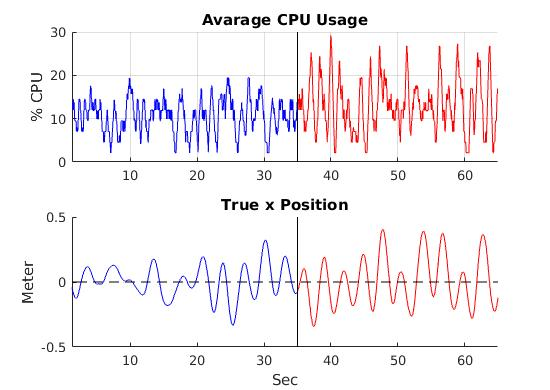
\includegraphics[width=100mm]{windPlot15.jpg}}
    \caption{This figure demonstrates how the reactive scheduler adapt to the changes in environmental conditions, in particular, to change of the wind. The upper part shows the average CPU usage during the flight, and the bottom is the true position at the same time. The first part of the flight, the left Blue graph, is a flight without any external wind, and in the rest of the flight, right red graph, the drone was exposed to artificial wind (using a fan). Note that when the drone is exposed to wind it uses more CPU to compensate for the disturbance.}
    \label{fig:windPlot}
\end{figure}

\section{Experiment Setup}
\label{sec:Experiment setup}

This Section present the technical details related to the implementation of the experiment in Section~\ref{sec:caseStudy}.

\begin{figure} %[htbp]
    \centerline{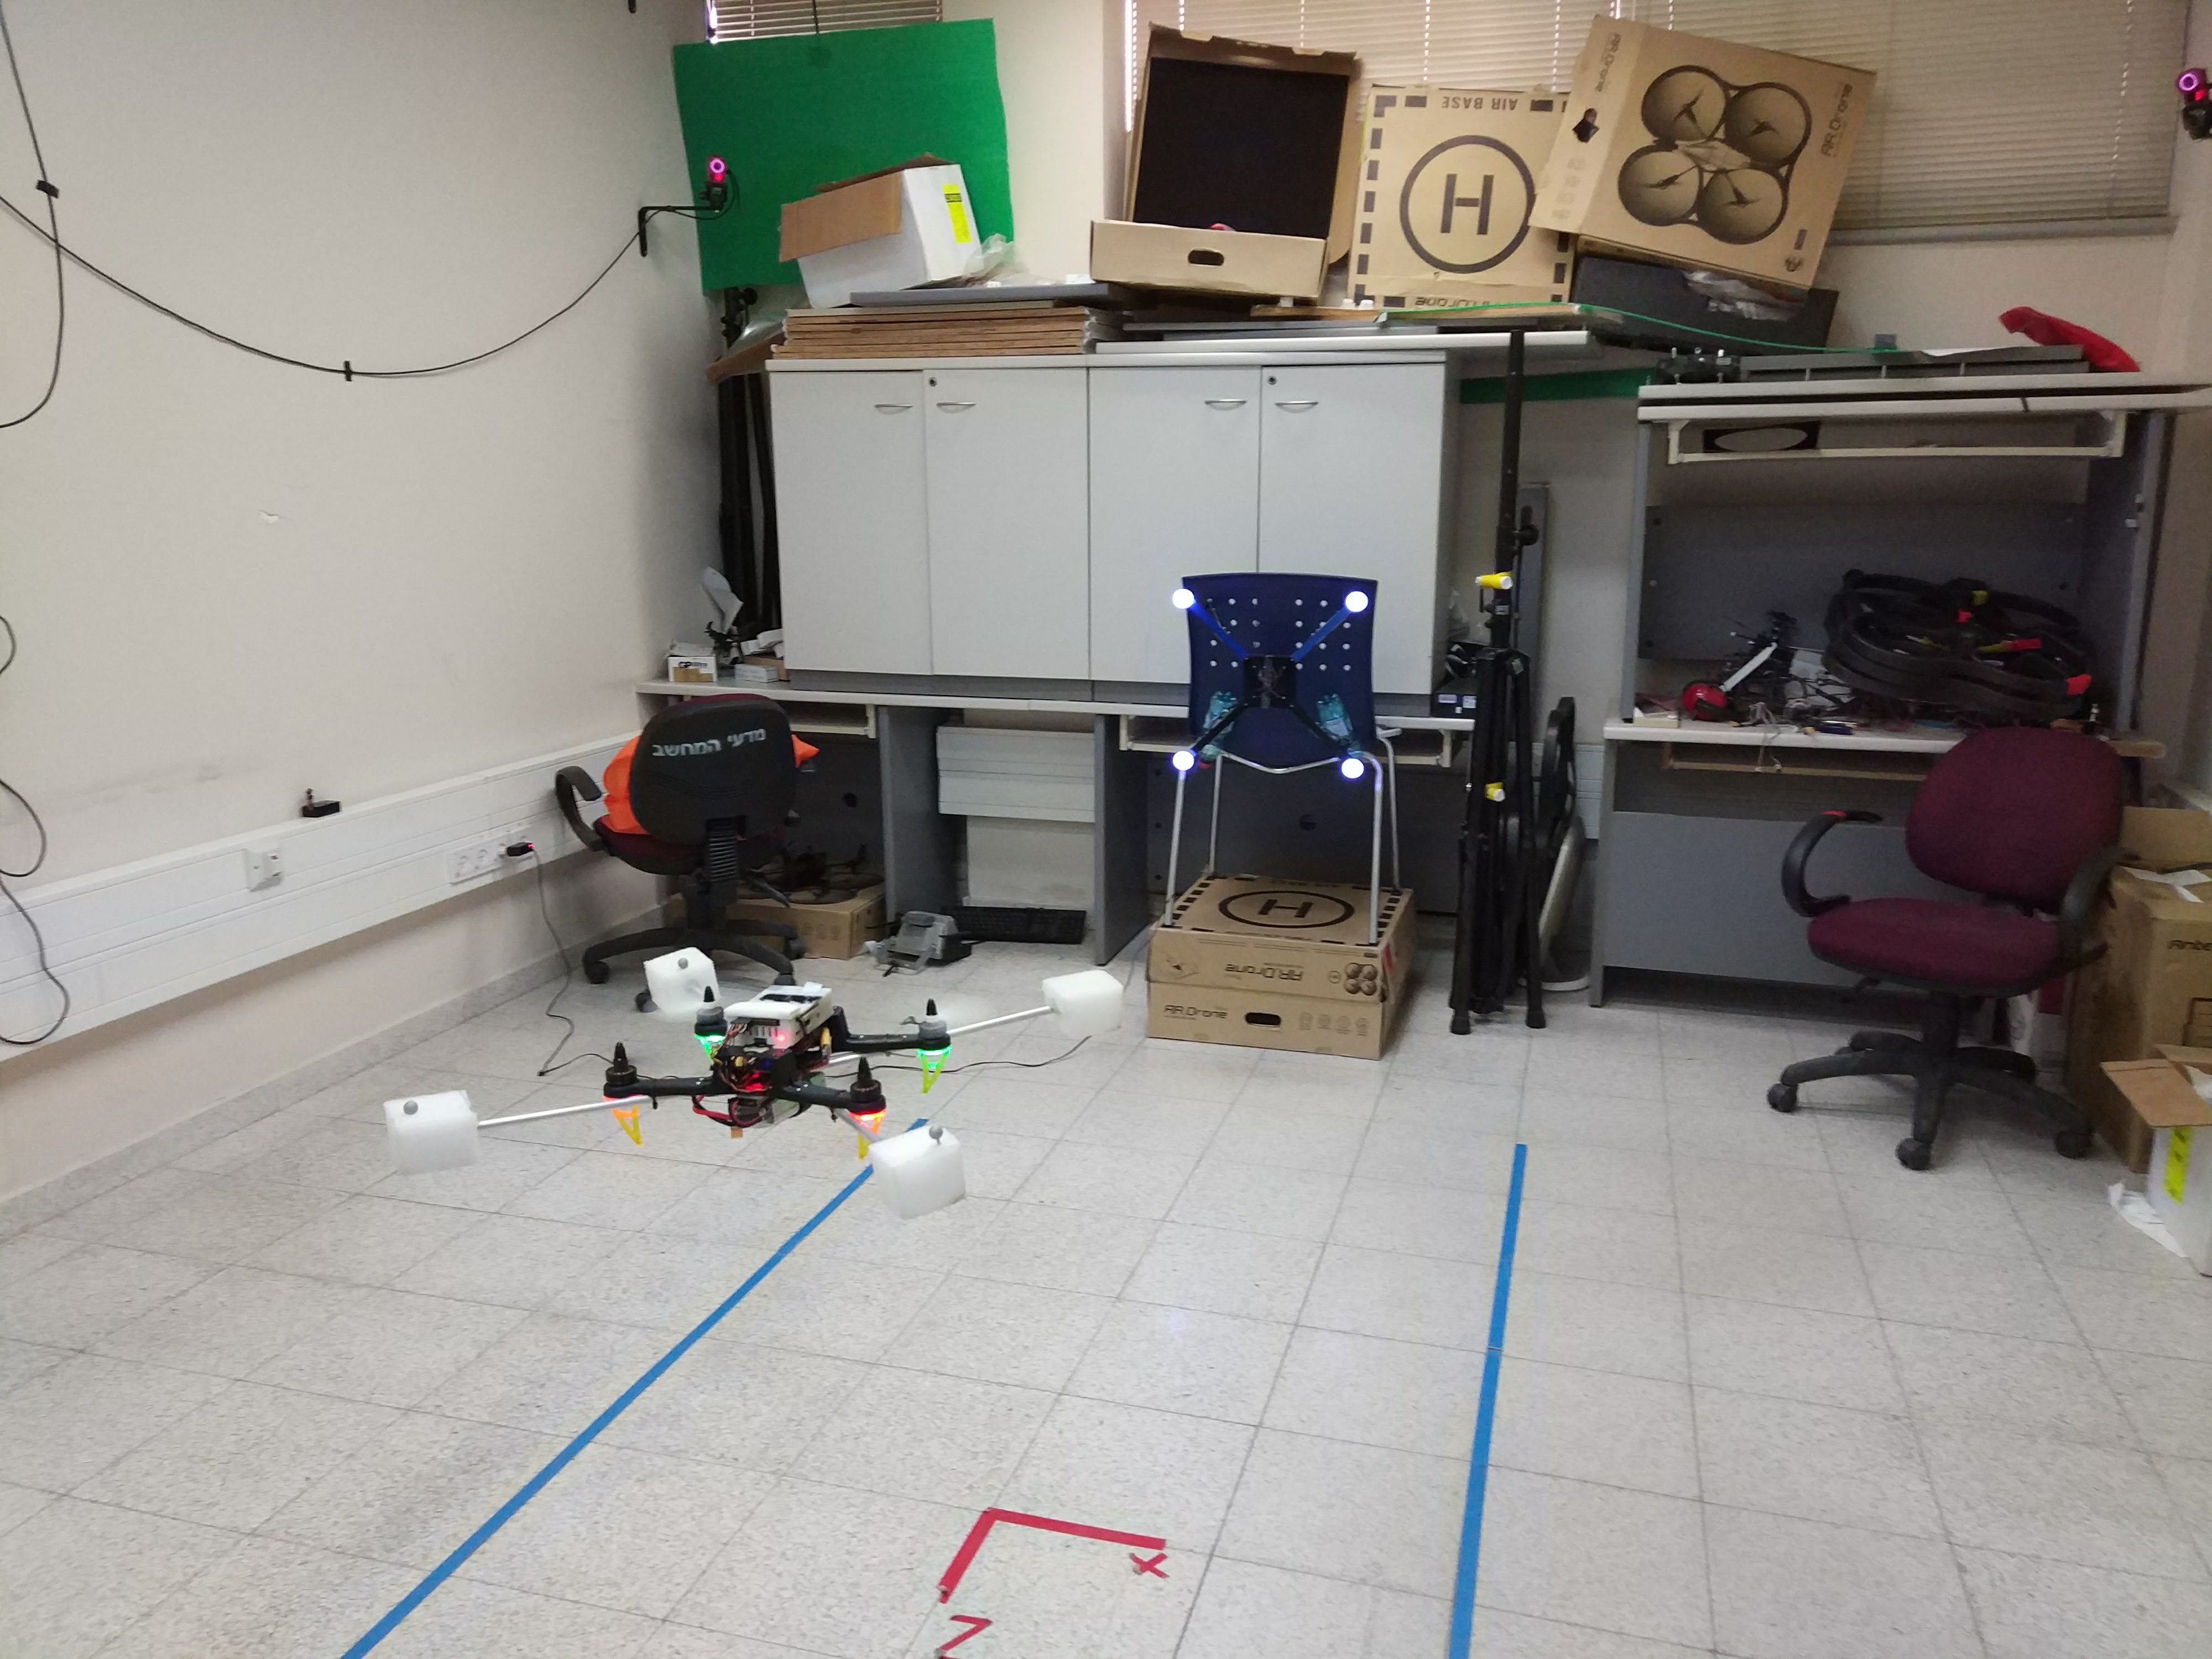
\includegraphics[width=100mm]{hover_in_lab.jpg}}
    \caption{This figure shows the drone hovering in front of the window during one of the experiments in our lab, the window in the tests is the four light balls in front of the drone.}
    \label{fig:hover_in_lab}
\end{figure}

\subsection{Hardware - the Quad-Rotor}
\label{sec:Experiment setup-HW}
% the hardware

In order to perform the experiments presented in Section~\ref{sec:caseStudy}, we used an of-the-shelf quadrotor, named \textit{Spedix-S250}, shown in Figure~\ref{fig:hover_in_lab} with improved flight controller: \textit{Raspberry-pi}, a single-board computer~\cite{raspberry}, with the \textit{navio2}~\cite{navio} shield.
\textit{Navio2} is extension board (shield) for the \textit{Raspberry-pi} platform. It provides the necessary interfaces such as remote control inputs and motors output, and it is equipped with on-board Micro Electro-Mechanical System (MEMS) sensors, such as rate gyros and accelerometers.
The software we used to controll the drone is ArduPilot Mega (APM) autopilot software~\cite{APM} with few modifications.


\subsection{The Controller Software}
We implemented the controllers and the schedulers as libraries for the ArduPilot Mega (APM) autopilot software~\cite{APM}.
APM architecture is very modular, the component are well separated but has well defined interface between them. This architecture allows us to easy replace, add, or modify the necessary parts.
The main changes in software that we made are, The addition of position sensing module based on image processing, and addition of our own flight-mode for handling the autonomous flight mission (in APM, flight-mode is the module responsible to apply the control law).
We also add position sensing module just for experiment references, this is module use OptiTrack in order to provide very precise position measurement. 

\subsection{Vision Based Position Sensor}
\label{sec:Experiment setup-cam}
% PiCam and drivers
As explained in Section~\ref{sec:caseStudy} we use vision-based sensor. This sensor first need to identify the window in front of the drone, and then produce position measurements relative to the window.
In order to identify the window we used a standard raspberry-pi camera module (V1) (see~\url{www.raspberrypi.org/documentation/hardware/camera/}), mounted in the front of the drone.
This camera can take pictures in different resolutions and at different frame rate.
The controller software implemented in C++, and we initially use the most common used driver for C++ called RaspiCam (see~\url{www.uco.es/investiga/grupos/ava/node/40}.
RaspiCam have two main difficulties for us:
\begin{enumerate}
    \item The raspberry-pi camera take a picture in a constant pre-define frame rate~\footnote{The constant pre-define frame rate is only when using ``vid'' mod which allows fast frame rate.}, this mean that if we want to grab an image the driver (RaspiCam) will wait till the next frame is taking. This approach is not suitable for real-time system.
    \item As describe in Section~\ref{sec:caseStudy} we need to switch image resolution many times during the flight, raspberry-pi camera resolution is defined only at initialization, therefore changing resolution of the camera results in significant delay, we need to initialize the camera again and wait till the camera is ready at the new resolution.
\end{enumerate} 

We solve the first difficulty by modifying RaspiCam driver. We add to RaspiCam the ability to notify the client when the next frame is ready, this way whenever a new frame is taken the callback function is called.
RaspiCam is open-source project, and we contribute to the project by adding this modification to the official RaspiCam code that is maintained in~\url{github.com/cedricve/raspicam}.

In order to overcome the second difficulty we try to take pictures at the high resolution and then resize by software (using OpenCV) to the desire resolution, this solution still add undesirable delay for each frame that is taking.
At the end, we create a new camera driver based on the work of Chris Cummings at~\url{robotblogging.blogspot.co.il/2013/10/an-efficient-and-simple-c-api-for.html}.
In this driver we use the internal GPU hardware of the Raspberry-py in order to resize the frame by hardware.
Using the ARM side libraries, \textit{userland}~(\url{https://github.com/raspberrypi/userland}). 
We construct network of four hardware resizers connected to four video ports, each resizer configure to a different resolution, and all are connected to the camera port (see Figure~\ref{fig:resize_ports}). 
Hardware operations takes relatively zero time to perform, and now each time we want to take a picture we can choose the image resolution by retrieving the image from the corresponded video port.

\begin{figure} %[htbp]
    \centering
    
    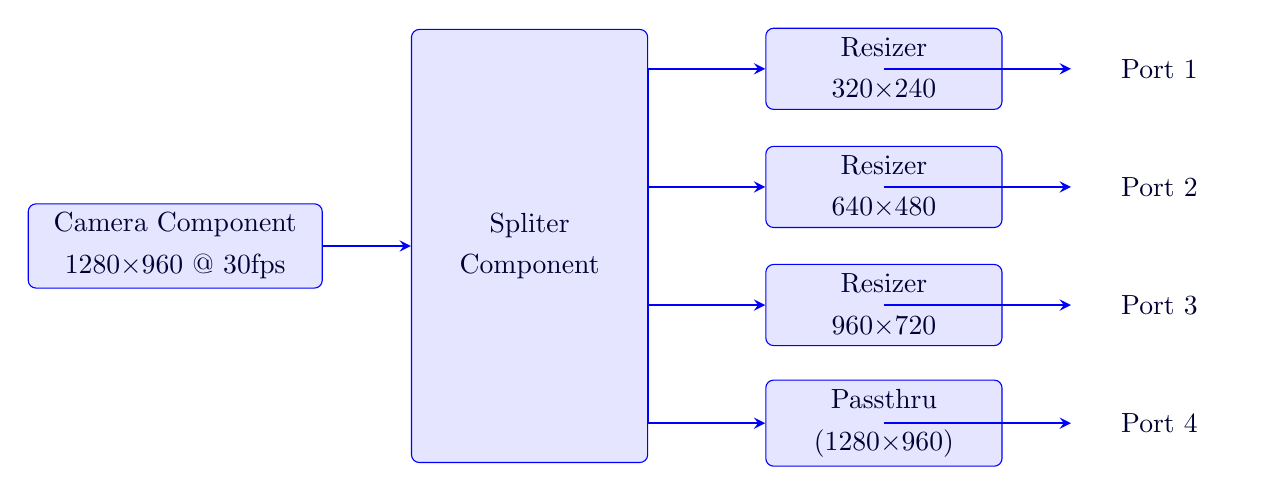
\begin{tikzpicture}[node distance=4.5cm]
        \node (cam) [recNodeB, text width=3.5cm] {Camera Component 1280$\times$960 @ 30fps};
        \node (sp) [recNodeB, text width=2cm, right of=cam, minimum height=5.5cm] {Spliter Component};
        \node (r1) [recNodeB, text width=2cm, right of=sp, yshift=2.25cm] {Resizer 320$\times$240 };
        \node (r2) [recNodeB, text width=2cm, right of=sp, yshift=0.75cm] {Resizer 640$\times$480};
        \node (r3) [recNodeB, text width=2cm, right of=sp, yshift=-0.75cm] {Resizer 960$\times$720};
        \node (r4) [recNodeB, text width=2cm, right of=sp, yshift=-2.25cm] {Passthru (1280$\times$960)};
        
        \draw [arrowB] (cam) -- node[above] {} (sp);
        \draw [arrowB] (sp.east) |- node[] {  } (r1.west);
        \draw [arrowB] (sp.east) |- node[] {  } (r2.west);
        \draw [arrowB] (sp.east) |- node[] {  } (r3.west);
        \draw [arrowB] (sp.east) |- node[] {  } (r4.west);
                
        \node (p1) [eNode, text width=2cm, right of=r1, xshift=-1cm] {Port 1};
        \node (p2) [eNode, text width=2cm, right of=r2, xshift=-1cm] {Port 2};
        \node (p3) [eNode, text width=2cm, right of=r3, xshift=-1cm] {Port 3};
        \node (p4) [eNode, text width=2cm, right of=r4, xshift=-1cm] {Port 4};
        
        \draw [arrowB] (r1) |- node[] {  } (p1);
        \draw [arrowB] (r2) |- node[] {  } (p2);
        \draw [arrowB] (r3) |- node[] {  } (p3);
        \draw [arrowB] (r4) |- node[] {  } (p4);
        
    \end{tikzpicture}
    
    \caption{This figure present the graphics processing unit (GPU) configuration we used for image resizing.}
    \label{fig:resize_ports}
\end{figure}

%vision algo
In the case-study, shown in Section~\ref{sec:caseStudy}, we always use the camera at 30 frames per second.
In order to simplify the image processing algorithm, we marked the four corners of the window with four illuminated balls (see Figure~\ref{fig:window_lights}). This allows us to apply a simple algorithm for corner recognition: 
look for a blob of burned pixels in the image, then calculate the ``center of mass'' of all those pixels as a window corner. Higher resolution give a more accurate measurement of corner ``center of mass'', but require more processing time.

% hanoch algo
Then we just perform the calculations presented in Section~\ref{sec:Observer Design} in order to extract the position measurements from the window corners.

\begin{figure} %[htbp]
    \centerline{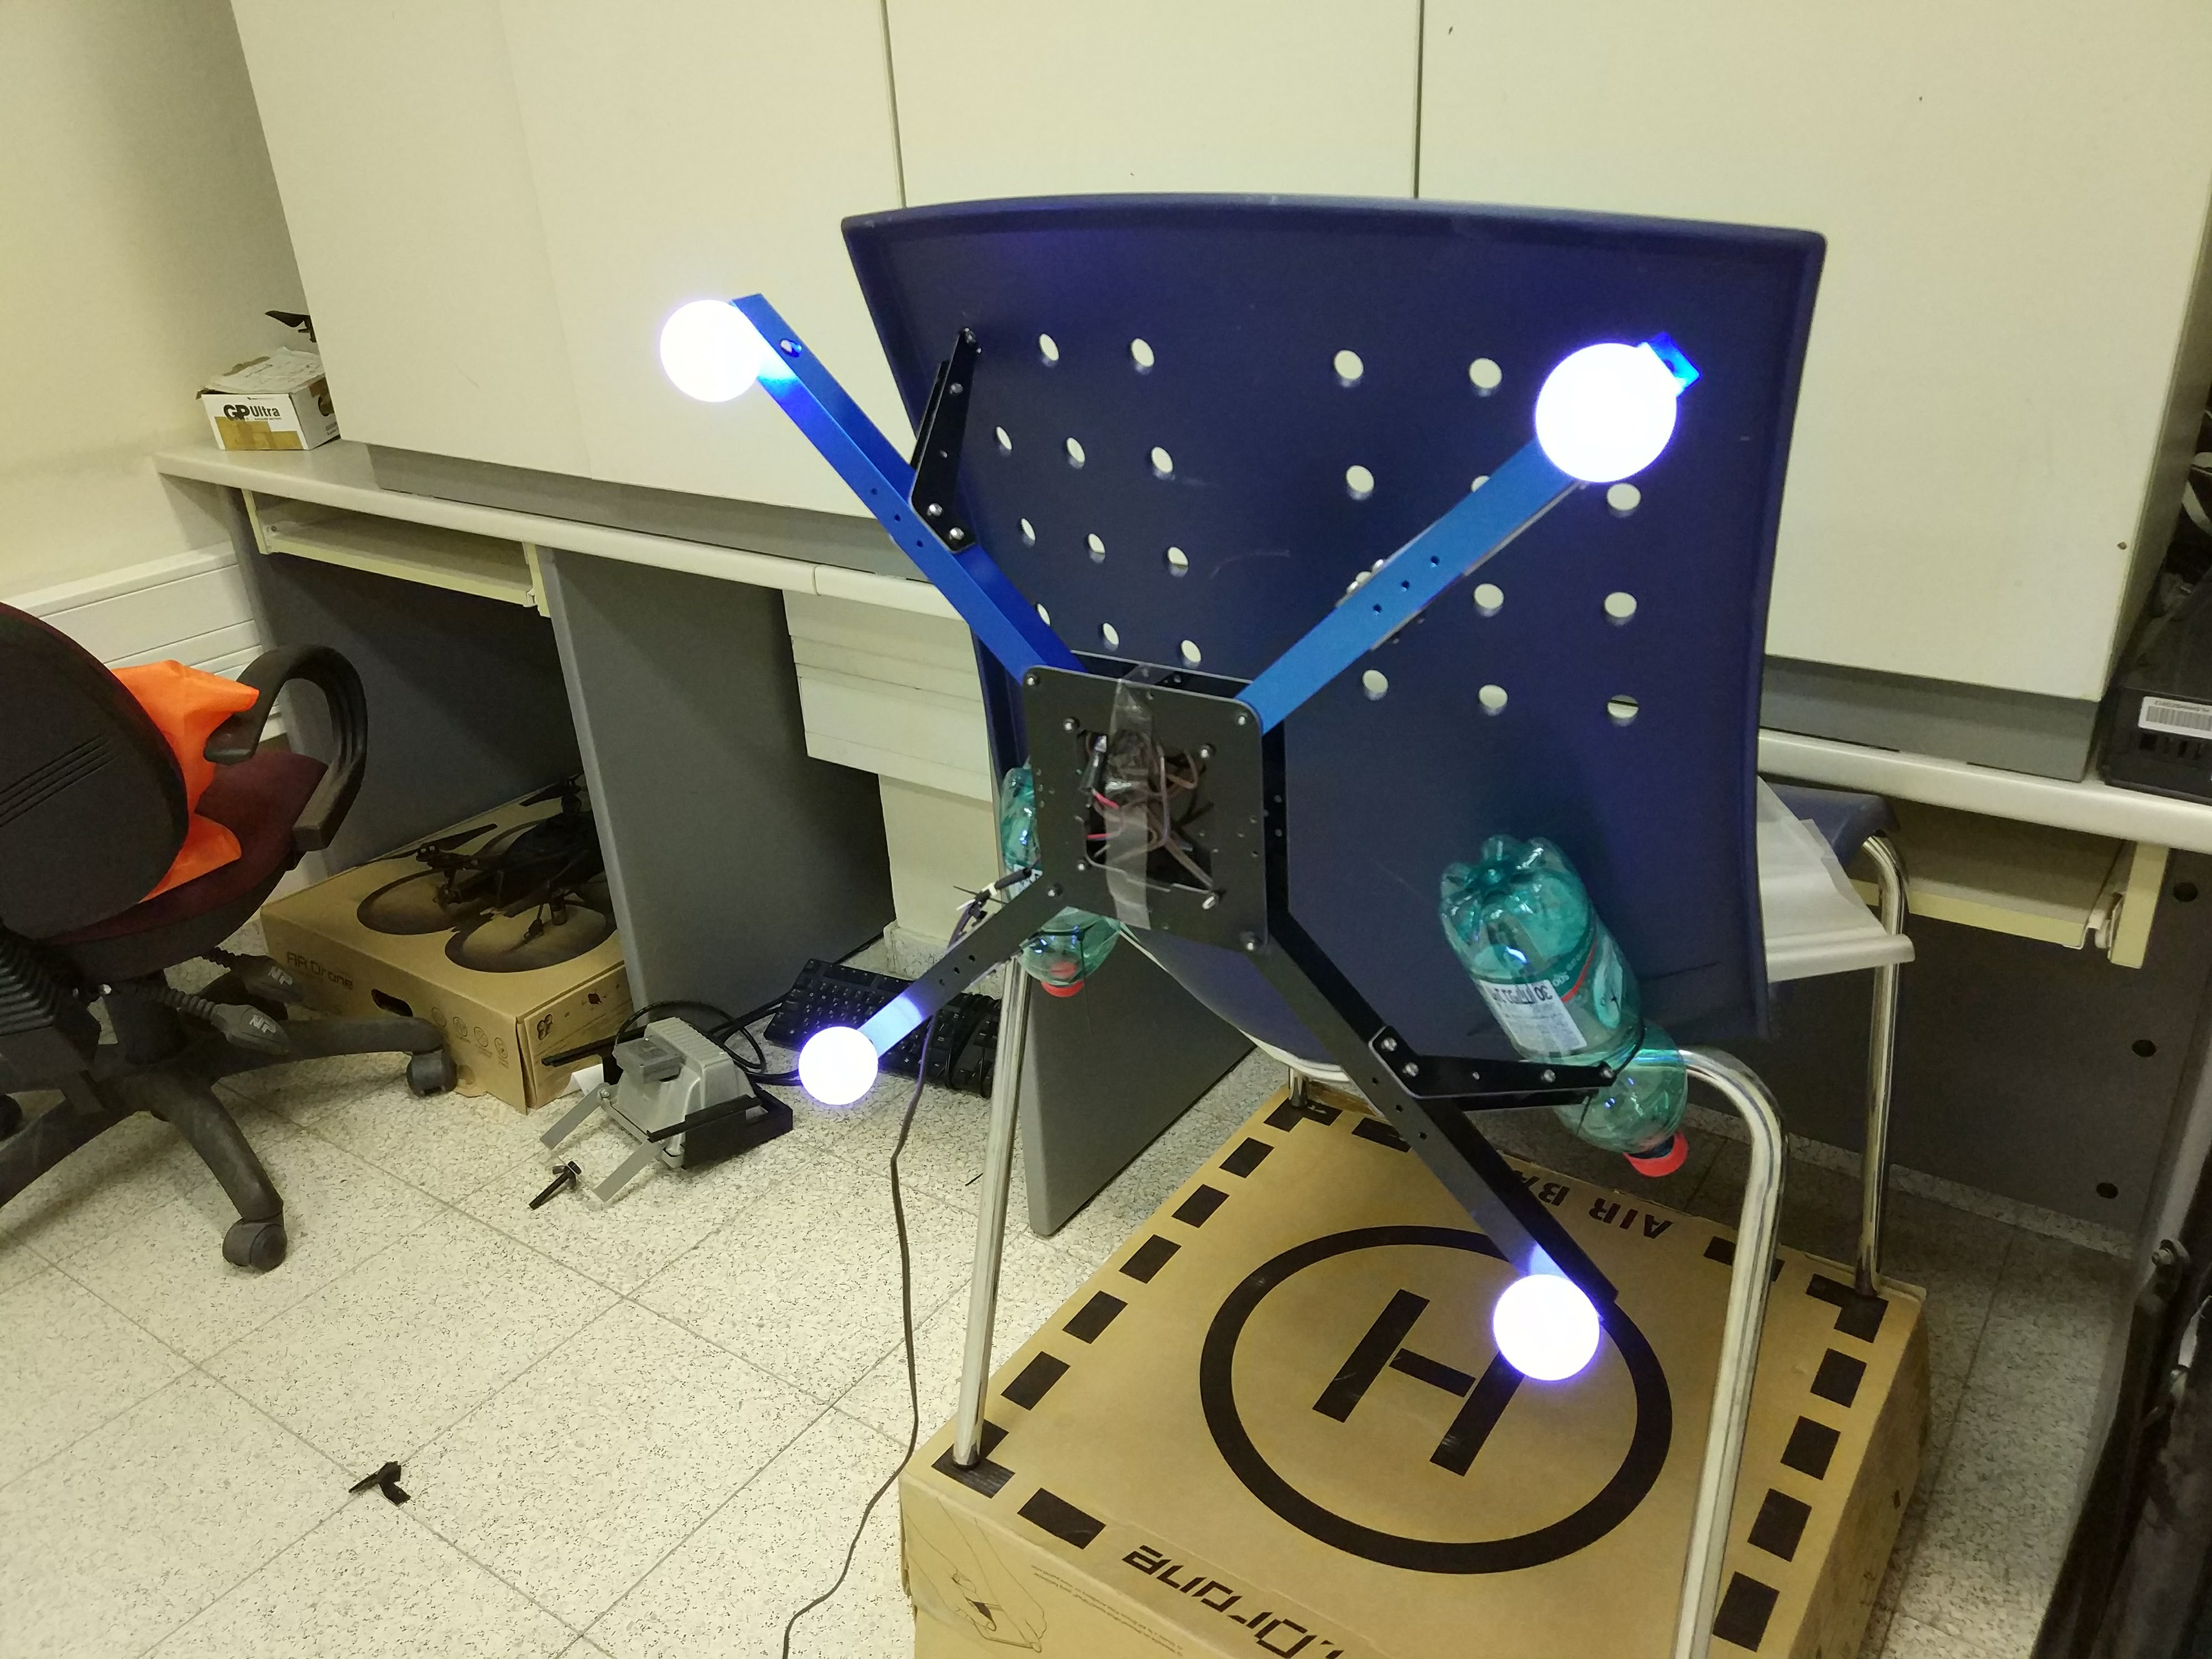
\includegraphics[width=70mm]{window_lights.jpg}}
    \caption{This figure shows the four light balls we used to represent the window during the experiment.}
    \label{fig:window_lights}
\end{figure}

\subsection{Reference Measurement with OptiTrack System}
\label{sec:Experiment setup-optitrack}
%OptiTrack
In order to evaluate the performance, we needed to know the accurate position of the drone during the flight. For this purpose, we used the \textit{OptiTrack} (\url{optitrack.com}) system 
consisting of an array of high-speed tracking cameras that provide low latency and high accuracy position and attitude tracking of the drone. The data from \textit{OptiTrack} system is sent over the client-server data streaming protocol \textit{NatNet}.

For best synchronization, we create a NatNet client library inside the APM code. This library allows the controller check anytime for the current state and log that information in parallel to the other controller parameters.
We also use the OptiTrack information in early stages of the research as the feedback of the controller before we use the Raspberry-pi camera.

\section{Scheduler Interface}
\label{sec:scheduler}
%The most common communication interface between scheduler and embedded real-time component, is by specifying a period, sometimes along with a deadline, which gives the frequency at which the component must be executed.
%The only requirement in those type of systems is that if the component is always executed exactly within the designed frequency (period), then the control objectives (e.g. stability) are met.
%%not directly in this article
%Specifying resource requirements using periods has advantages due to simplicity and analyzability, but has limited expressiveness, as elaborated in~\cite{RTComposer}. 
%%For example, a specification such as “execute the component every 5ms” does not say whether the scheduler should or should not execute it more frequently if enough computing resources are available, and if a component has multiple, say, for different control tasks, each needing a different period, the requirement cannot be naturally captured by a single period.
In Section~\ref{sec:architecture} we explained how automata allow for rich component specification for reactive scheduling. While the automata used in the experiments where crafted by hand without automatic composition, we outline in this section how to formally create and compose automata using \buchi game theory. The formalisms described below  allow for automating the composition and the schedule generation using tools such as GOAL~\cite{goal}.

In our framework, similarly to most traditional real time systems, the resource is allocated in discrete \textit{time slots} of fixed duration in the style of time-triggered architecture~\cite{RTComposer}. A typical software control system consists of multiple tasks that need to be taken care of simultaneously in order to control the system.
Each task is implemented by one or more subroutines (code functions). We suggest to design control system in the \textit{component} level, where each component corresponds to a specific task in the system consisting of all the subroutines of the task along with a \buchi game specify how the task subroutines should be executed. This is formalized in the following definition:

\begin{dfn}
    A component is a pair $\langle T,G\rangle$ where $T$ is a set of subroutines (representing, e.g., procedures of a class in C++) and $G=\langle A,\langle P_{schd}, P_{env}\rangle \rangle$ is a generalized B{\"u}chi game (GNBG), over a generalized \buchi automaton $A= \langle Q,\Sigma,\Delta,q_0,\mathcal{F} \rangle $ (see Section~\ref{sec:GNBG}), such that:
    \begin{enumerate}
        \item The \textit{alphabet} is $\Sigma = 2^{T} \cup \R^n$ where $n$ is the number of scheduler feedback variables in the system (real numbers that the scheduler can base its decision on).
        \item 
        Alternating turns with different parts of the alphabet:
       	The transitions of $A$ are of the form: $q_{schd} \xrightarrow[]{\sigma_{T}} q_{env}$ where $q_{schd} \in P_{schd}, q_{env} \in P_{env},$ and $\sigma_{T} \subseteq T$ (called  ``scheduler'' transitions ),  or of the form $q_{env} \xrightarrow[]{\sigma_{e}} q_{schd}$, where $q_{schd} \in P_{schd}, q_{env} \in P_{env}$, and $\sigma_{e} \in \R^n$ (called ``environment'' transitions).
        \item The environment plays first: $q_0 \in P_{env}$.
    \end{enumerate}
\end{dfn}

The \buchi game, $G=\langle A,\langle P_{schd}, P_{env}\rangle \rangle$, of a component is a game of the scheduler against the environment. It represents the interaction of the controller with the environment in the real world.
The game goes as follows: before each time slot the environment player ($P_{env}$) plays first and takes the transition $q_{env} \xrightarrow[]{\sigma_{e}} q_{schd}$ signaling that  the observation values at the beginning of this slot is $\sigma_{e} \in \R^n$.
Then, the scheduler needs to choose a transition $q_{schd} \xrightarrow[]{\sigma_{T}} q_{env}'$ and to execute all the tasks in $\sigma_{T}$.
The environment transition represents the evolution of the system state during the previous time step, caused by the actuators and the environment noise. The scheduler transition is the scheduler reaction to this state evolution.
This simultaneous walk over the game automata ($A$) creates infinite path $p_{\omega} = q_0 , q_1, \dots$,
and the scheduler goal is to pass through (all sets of) accepting states infinitely many times during the execution, formally, the goal is a path that $\forall F \in \mathcal{F} : \inf (p_{\omega}) \cap F \ne \emptyset$.
In other words, if the word $\omega = \vec{y}_1 , T_1, \vec{y}_2, \dots $ created by this simultaneous walk over the game automaton $A$, is an accepting world (if $\omega \in \mathcal{L}_{\omega}(A)$), then the scheduler is the winner, and the resulting schedule execution achieves the component objectives.
Note, the scheduler feedback variable (or observations) vector, $\vec{y} \in \R^n$, may includes state variables and internal variable of the components.

This interface is demonstrated in Figure~~\ref{fig:exampleGame} in the context of a vision based sensor component of a robot. 
The component we focus on here estimates the robot position using a camera. It has two operation modes: high (H) or low (L) accuracy.
The variable $y$ is the estimated position. In this example the component requirement is to ensure that $y$ never exceeds one (there is a cliff that starts at $y=1$).

\begin{figure} [h]
    \centerline{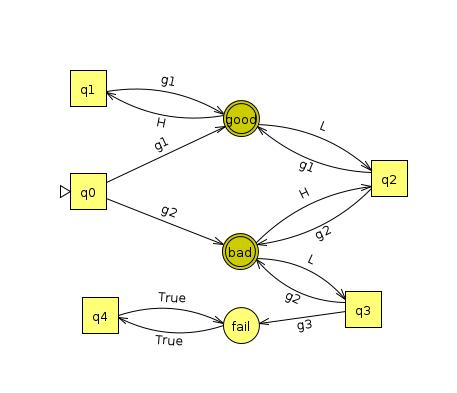
\includegraphics[width=100mm]{gameExample.jpg}}
    \caption{Example of a game for vision based sensor component of a robot.
        The robot must maintain position of $y \le 1$.
        The tasks $H$ and $L$ are high accuracy and low accuracy position measuring tasks respectively, and
        $g1$ refer to every observation that $y \le 0.5$, $g2$ refer to $0.5 < y \le 1$ and $g3$ refer to $1 < y$. }
    \label{fig:exampleGame}
\end{figure}

%\subsection{Component Games Composition}
As we said a typical system composed of multiple components that need to be executed simultaneously by the same processor.
Each component have its own game (its own requirements), therefore we will construct a composed component that correspond to all the system components together, then the scheduler have only one component, with only one game to win for scheduling all the components.
Let's define composition of the components, that preservative the logic and correction of its composed components.

\begin{dfn}
    The composition of the components $C_1=\langle T_1, \langle A_1, \langle P_{schd}^1, P_{env}^1\rangle\rangle\rangle$ and $C_2=\langle T_2, \langle A_2, \langle P_{schd}^2, P_{env}^2\rangle\rangle\rangle$ is the component $C_c = C_1 \times C_2 = \langle T_1 \cup T_2, \langle A_c, \langle P_{schd}^1 \times P_{schd}^2, P_{env}^1 \times P_{env}^2 \rangle\rangle\rangle$ where $A_c= \langle Q_1 \times Q_2,(T_1 \cup T_2) \times \R^n,\Delta_c,Q_0^1 \times Q_0^2,\mathcal{F}_1 \cup \mathcal{F}_2 \rangle$ is a product of $C_1$ and $C_2$ and 
    \begin{enumerate}
        \item Environment transitions: $\forall y \in \R^n, s_1 , s_1' \in Q_1, s_2 , s_2' \in Q_2$:
        $\langle s_{1} s_2 \rangle \xrightarrow[]{y} \langle s_{1}' s_2' \rangle \in \Delta_c$
        if and only if 
        $s_{1} \xrightarrow[]{y} s_{1}' \in \Delta_1$ and $s_{2} \xrightarrow[]{y} s_{2}' \in \Delta_2$.
        \item Scheduler transitions: $\forall T_1' \subseteq T_1,T_2' \subseteq T_2$ , $s_1 , s_1' \in Q_1, s_2 , s_2' \in Q_2$:
        $\langle s_{1} s_2 \rangle \xrightarrow[]{T_1' \cup T_2'} \langle s_{1}' s_2' \rangle \in \Delta_c$
        if and only if         
        $s_{1} \xrightarrow[]{T_1'} s_{1}' \in \Delta_1$ and $s_{2} \xrightarrow[]{T_2'} s_{2}' \in \Delta_2$.
    \end{enumerate}
\end{dfn}

Note: components composition is defined for compose two components, but we can compose all the system component, $C_1 , ... , C_m$, one by one: $C_c = (\cdots((C_1 \times C_2) \times C_3 ) \times \cdots \times C_m)$.

%\subsection{Add Resources Limitation}
In addition to the component requirements (requirements from control objective) we also have resources requirements, we have limited resources (limited CPU abilities) that need to be taking in account.
Resources requirements are reflected as limited time slot capacity, each subroutine (procedure) take some time to perform but the slot is limited in time.
For example, two subroutines $t_1$ and $t_2$ that require 1.5 millisecond each to execute, cannot be executed in two millisecond time slot.
We will enforce the slot size with a special and simple component $C_{resource}$ that can be generated automatically as follows:
assuming we know the maximum duration of each subroutine of the components in the system (it can be result of analyzing, testing, or manually pre-defined) we construct component with the tasks set $T$ that is union of all the subroutines in the system, and the game ($G_{resource}$) is as demonstrate in Figure~\ref{fig:C_resource} with one state for environment player (square state) and one for the scheduler (circle state), the environment have no limitations but the scheduler can execute only set of tasks that not exceeds the time slot.

\begin{figure} [h]
    \centerline{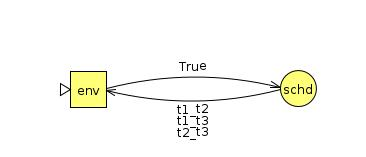
\includegraphics[width=80mm]{reasourceGame.jpg}}
    %\subfile{./goal/reasourceGame.tex}
    \caption{Example of a game for resource component that do not allows to exceed a time slot. 
        In this example $T = \left\{ t_1 , t_2 , t_3 \right\}$, the execution time of each task $t_i$ is half of a single time slot, therefore it is not possible to execute more than two tasks at the same time slot, but there is no limitation on the environment ($\vec{y}$).
        Square state is an environment player state and round state belong to the scheduler.  }
    \label{fig:C_resource}
\end{figure}

Finally, the resource component is composed with all the rest components of the system resoult in the schedule component $C_s = C_{resource} \times C_c$.

%\subsection{Wining the Game - Find the Strategy}
The component $C_s$ aggregates all the system constrains, in order to successfully schedule the system, we need to find a ``wining'' strategy $A_{strategy} \in NBA$ for the scheduler.
$A_{strategy}$ is in fact, a reduction of the game automaton $A_s = \langle Q_s ,\Sigma,\Delta_s, Q_0, \mathcal{F}_s \rangle$ of $C_s$. It is contained all the environment transitions in $A_s$, but only the scheduler transitions that allays can lead to a winning of the scheduler player, that is, runs that we visit infinitely times a state of every color $F' \in \mathcal{F}_s$.
Example of such strategy is shown in Figure~\ref{fig:exampleGameStrategy}, the blue partial automaton is the scheduler wining strategy for the game presented in Figure~\ref{fig:exampleGame} discussed before.
We call this winning strategy a guarded automaton.

\begin{figure}[h]
    \centerline{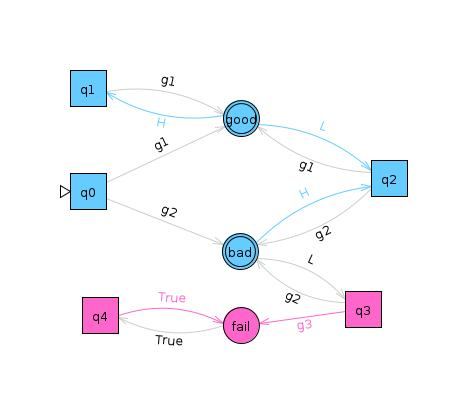
\includegraphics[width=100mm]{gameExampleSolved.jpg}}
    \caption{A strategy solution for the game presented in Figure~\ref{fig:exampleGame}.
        Blue states are all the states which the scheduler have a wining strategy from them, blue transitions are the needed scheduler reaction to win the game.
        Note: if the initial state is blue then the system is schedulable.}
    \label{fig:exampleGameStrategy}
\end{figure}

%\subsection{Execution of the scheduler}
The complete operation of the scheduler is described by the pseudo code~\ref{code:schedulerPrepare}.
Every time the system is executed, the scheduler construct the strategy automaton $A_s$, and then just walk through the strategy as describe by the pseudo code~\ref{code:scheduler}. 
%The time is divided into segments of equal length, called ``time step''.
%At the beginning of each time step the current automaton state is environment player state, so we pick the %{continue verbal explanation of the pseudo cod }


\begin{algorithm}[h]
    \caption{Scheduler start up procedure}
    \begin{algorithmic}[1]
        \Procedure{ScheduleStartUp}{$C_1, \dots , c_m$} \Comment{schedule the components $C_1, \dots , c_m$}
        
        \State $C_c$ $\gets$ \Call{Compose}{$C_1, \dots , c_m$}
        \State $C_{resource}$ $\gets$ \Call{CreateResourceComponent}{$C_1, \dots , c_m$}
        \State $C_s$ $\gets$ \Call{Compose}{$ C_c , C_{resource}$}
        
        \State $A_s$ $\gets$ \Call{FindWiningStrategy}{$C_s$}
        
        \If {$A_s$ is not empty}
        \State \Call{Schedule}{$A_s$}  \Comment{ start to run the system}
        \EndIf
        
        \EndProcedure
    \end{algorithmic}
    \label{code:schedulerPrepare}
\end{algorithm}

\begin{algorithm}[h]
    \caption{Scheduler run-time operation}
    \begin{algorithmic}[1]
        \Procedure{Schedule}{$A_s$} \Comment{schedule the system with strategy automaton $A_s$ }
            %\State \Call{Validate}{$A_s$} \Comment{validate that $A_s$ is wining strategy}
            \State $cur\_state \gets$ \Call{Initial}{$A_s$} \Comment{start with the initial state}
            
            \Statex
            \Loop 
                \State $\vec{y} \gets \Call{getStateVars}$  \Comment{the scheduler observations}
                
                \State $cur\_state \gets$ \Call{Next}{$cur\_state$ , $\vec{y}$} \Comment{take the environment transition for $\vec{y}$ }
                %\If {$cur\_state == None$}
                %    \State Exit \Comment{unexpected $\vec{y}$ value, fail to proceed}
                %\EndIf
                
                %\Statex
                \State $\langle From , Tasks, To \rangle$  $\gets$ \Call{Next}{$cur\_state$} \Comment{take scheduler transition}
                %\State $Tasks \gets$ \Call{tasks}{$\delta$}
                
                \ForAll{ $t \in Tasks$} \Comment{execute all the tasks defined by the transition}
                    \State \Call{Execute} {$t$}
                \EndFor
                
                \State $cur\_state \gets$ $To$ \Comment{take the transition}
                
                %\Statex
                \State Wait till next time step
                
            \EndLoop
        \EndProcedure
    \end{algorithmic}
    \label{code:scheduler}
\end{algorithm}


\subsection{Correctness of Scheduler Operations}

\begin{dfn}
    A component $C_i$ is \textbf{complete} if for each $t_1, \dots, t_m \subseteq T_i$, $\vec{y}_1, \dots , \vec{y}_m \in \R^n$ and $q_e \in P_{env}$ such that there is a path from $q_0$ to $q_e$ with the word $w= \vec{y}_1 , t_1 , \vec{y}_2 , t_2, \dots , \vec{y}_{m}, t_m$ we have that for each $\vec{y}_{m+1}$ that can be observed after any run of the system that corresponds to this word (i.e., a run where after each observation $\vec{y}_j$ we scheduled $t_j$) there is a transition from $q_e$ labeled with $\vec{y}_{m+1}$.
\end{dfn}

\begin{dfn}
    \label{thm:well-formed}
    A component $C_i= \langle T_i, \langle A_i, \langle P_{schd}^i, P_{env}^i\rangle\rangle\rangle$ is \textbf{well-formed} if it is complete, and in any execution whose observations and task schedules constitute a word $\omega \in \mathcal{L}(A_i)$, the component achieves its control objectives.
\end{dfn}

\begin{claim}
    \label{thm:valid_composition}
    If $C_1=\langle T_1, \langle A_1, \langle P_{schd}^1, P_{env}^1\rangle\rangle\rangle$ and $C_2=\langle T_2, \langle A_2, \langle P_{schd}^2, P_{env}^2\rangle\rangle\rangle$ are a well-formed components then their composition $C_c=C_1 \times C_2$ is also a well-formed component.
\end{claim}
\begin{proof}
    \begin{enumerate}
        
        % all posible y
        \item $C_c$ is a complete component: Assume that after we get to state $\langle q_1 , q_2 \rangle \in P_{env}^1 \times P_{env}^2$ we may observe $\vec{y}$, then because $C_1$ is complete there is a transition $q_1 \xrightarrow[]{\vec{y}} q_1'$ and same for $q_2 \xrightarrow[]{\vec{y}} q_2'$ in $C_2$, therefore by the composition definition $A_c$ contains the transition $\langle q_1 , q_2 \rangle \xrightarrow[]{\vec{y}} \langle q_1' , q_2' \rangle$
        
        \item $C_c$ is a well-formed component: by the definition of composition the word $\omega= \vec{y}_1 , t_1 , \vec{y}_2 , t_2, ... \in \mathcal{L}(A_c)$ if and only if there exist words $\omega_1= \vec{y}_1 , t_1^1 , \vec{y}_2, t_2, ... \in \mathcal{L}(A_1)$ and $\omega_2= \vec{y}_1 , t_1^2 , \vec{y}_2 , t_2^2, ... \in \mathcal{L}(A_2)$ such that $t_i = t_i^1 \cup t_i^2$. 
        Therefore, for each $\omega = \vec{y}_1 , t_1 , \vec{y}_2 , t_2, ... \in \mathcal{L}(A_c)$ a system execution that before each time slot $j$ observe $\vec{y}_j$ and then execute the tasks $t_i$ in that slot, is in particular execute $t_i^1$, and because $\omega_1= \vec{y}_1 , t_1^1 , \vec{y}_2 , t_2, ... \in \mathcal{L}(A_1)$, $C_1$ achieve its control objectives. Similarly, $C_2$ also achieve its control objectives with $\omega$, then $\omega$ is a system execution that satisfies the requirement of the system components.
        
    \end{enumerate}
\end{proof}

\begin{dfn}
	A system is \textbf{schedulable}, if for any possible behavior of the environment (measurements that it may produce), there is a way for the scheduler to assign tasks such that all components achieve their control objectives.
\end{dfn}

\begin{claim}
    If $C_1,\dots , C_m$ are a well-formed components and there is a non-empty wining strategy for the composed component $C_s=C_1 \times \cdots \times C_m \times C_ {resource}$, then the system defined by $C_s$ is schedulable.
\end{claim}
\begin{proof}
    First note that $C_{resource}$ is a well-formed component:
    The only environment state of $A_{resource}$ accept all $\R^n$ for the observations, therefore $C_{resource}$ is complete. 
    And the only requirement from $C_{resource}$ is that no time step is never exceeded it length, this is guarantied by the contraction of scheduler transitions in the resource component, therefore  $C_{resource}$ is a well-formed component.
    All components $C_1 , C_2 , .. , C_m$ and $C_{resource} $ are a well-formed components then by Claim~\ref{thm:valid_composition} $C_s $ is also a well-formed component.
    
    Assume there is a wining strategy for $C_s$ then the scheduler that random walk trough the wining strategy automaton, and operate as elaborate in Algorithm~\ref{code:scheduler} is:
    \begin{enumerate}
        \item Never get stuck: $C_s$ is complete so each environment state of its automaton, $A_s$, have transition for any possible observation,
        therefore we never get stuck at environment state.
        %and any strategy of scheduler must keep all environment transitions therefore the execution never get stuck at environment state. 
        And each scheduler state in the strategy have at least one outcome transition because if not then the strategy is not a wining strategy. 
        
        \item All the transitions of the component $C_{resource}$ game have a task sets that, even at the worst case, never exceeds a single time step. 
        $T_{resource}$ contains all the system components subroutines, therefore, $C_s$ also do not contain tasks sets that exceeds a single time step.
        %, therefore a schedule of a longer tasks set is not possible in algorithm~\ref{code:scheduler}.
        
        \item The system achieves the control objectives: The component $C_s$ is well-formed,and the random walk of algorithm~\ref{code:scheduler} is constructing a word $\omega \in \L(C_s)$, therefore, by the definition of well-formed compnents (Definition~\ref{thm:well-formed}), the run of algorithm~\ref{code:scheduler} that construct the word $\omega$ achieves the system control objectives.
    \end{enumerate}
\end{proof}

\subsection{Some More Words on the Implementation}

% finite space by discretization of observations (Merav)
We defined the alphabet of a component game to be $\Sigma = T \cup \R^n$, but $\R^n$ is of course infinite set so we can not store the game in the finite storage of the control computer.
We need to transfer the infinite continues space $\R^n$ to discrete space, without loosing any flexibility.
In practice, we do not need to create explicit transition for every possible value of the observation $\vec{y}$.
The environment transitions are annotated with values intervals, which define a subset of $\R^n$, for example the transition $q \xrightarrow[]{-1<y_1<1, -1<y_2<1, \dots , -1<y_n<1 } q'$ can be used for every $\vec{y}' = \langle y'_1, \dots , y'_n \rangle \in \R^n$ such that $\forall 1 \le i \le n : -1 < y'_i < 1$.
With this annotation we can store infinite games (and strategies solutions) in a small computer.

In addition, for successfully calculate the automata operations, such as, compose games with intersect intervals on the transitions, we need to proper define the intervals.
The solution, which elaborated in details in the work of Merav~\cite{Merav}, is to collect all the scalar numbers in all the component games, and define interval for every two adjacent scalars. Then the alphabet contain only tuples of $n$ intervals for every $n$ intervals combination. 


% game solver - GOAL
With the above discrete alphabet, we can perform most of the automata operations with common automata algorithms and existing automata tools. 
In this thesis we used the GOAL tool~\cite{goal} for composing games, finding wining strategy for a game and other analysis such as emptiness and simplification of automata.

% preparation time vs run time
An important characteristic of task scheduler is run time, sometimes referred to as switching time.
The scheduler must consume minimum of CPU time. In the proposed methodology the scheduler need to perform many automata and game related operations, which can take significant processing time to calculate.
In practice, all those calculations need to be performed only once for a system. 
We can perform all those calculations once in the compilation time, and then the scheduler only need to walk through the strategy automaton, which require only constant amount of calculations before every time slot.


\section{Related Work}

This thesis is mainly based on the RTComposer paper~\cite{RTComposer} and the followed work, GameComposer, of Merav~\cite{Merav}.
In this thesis like in RTComposer we present a framework for design cyber-phisical systems with dynamic scheduling for real-time.
RTComposer presents so called component-based framework in the sense that a single component correspond to a single control loop in a complex cyber-phisical system.
Each component has a clearly specified interface that includes method for sensing, method for actuation, and additional computational methods that can be executed between the time of sensing and actuation.
Each component have requirement specification given by finite automaton over infinite words, every infinite sequence over the automaton specifies, for every time slot, the set of computational methods to invoke in that slot.

In this thesis we also continue the use of automata based scheduler, automata specification is expressive, analyzable, and composable specification framework as stated in Section~\ref{sec:architecture} and in RTComposer paper~\cite{RTComposer}.
After reviewing few embedded control systems, we conclude that RTComposer component design can be limiting. 
Most control systems have multiple control loops but they may have shared tasks.
An example for such system is shown in Section~\ref{sec:caseStudy}, there is a three dimensional flying machine with four control loops (pitch, roll, yaw and throttle) that share a single image based sensing task along with some private tasks like compass sensor used only by the yaw control loop.
%As elaborate in section~\ref{sec:scheduler} we define component as ...
In this work, unlike RTComposer, we loosen the definition of a component, and remove the separation of sensing and actuation methods, and remains only with computational methods, then a component is not necessarily correspond to a single control loop (see Section~\ref{sec:scheduler}). 
In this way we can define a single component for the vision based sensing, ans 4 additional components for pitch, roll, yaw and throttle control loops that gets information from the vision component.

% game composer inspiered by merav for reactive scheduling
% merav concentrated in automata and exponential stabilisation and develop great tools
The GameComposer by Merav~\cite{Merav}, similarly to this thesis, extends RTComposer by adding the ability of ``reacting'' to the environment.
Inspired from GameComposer we use \buchi game as the main component specification, which allows the scheduler to make scheduling decision based on the current characteristics of the plant.
Those games extends the specification automata of RTComposer with the addition of environment player and environment transitions (see Section~\ref{sec:scheduler}).
The environment may help or interfere with the control operation, we manage to improve the controller performance by consider this environment influence, see Section~\ref{sec:results}.
General speaking Merav focuses on the technical aspects of the scheduler and automata related algorithms.
This work focus on the integration of the automata based scheduling in a cyber-phisical systems.

% rt stabilization vs kalman-filter scheduling
RTComposer also describes techniques for generate the specification automata. For example, automata for a traditional periodic tasks, or automata that guaranty stability objectives for a given linear switched system.
Those RTComposer techniques are all techniques for offline scheduling and they can be also applied in our proposed framework.
In this work we present online techniques that can take in to account the current state of the system.
We show how to use information from the classic Kalman fiter observer (Section~\ref{sec:simulation}) and a simplest linear version with complementary filter (Section~\ref{sec:Analysis}.
We manage to extract an estimation of the process and measurement errors from the filter, and schedule sensing tasks base on this estimation.


%TODO - online composition


%TODO - we present real life experiments or maybe in conclusion
%TODO - micro / macro scheduler


% hanoch
The case-study in this thesis, presented in Section~\ref{sec:caseStudy}, \todo{ask hanoch for reference} is based on the work of Hanoch~\cite{Hanoch ??}.
Hanoch present an iterative technique for calculating the position and attitude of the drone relative to a window.
In this technique the drone is equipped with a camera pointed to the front of the drone, the camera is capable of photographing a window and finding the four corners of the window in the image surface.
Hanoch's algorithm takes the position of the corners and calculate the position and attitude relative to the window.
In the case-study of this thesis we control and regulate the position and attitude of the drone (see Section~\ref{sec:Observer Design}) using the same techniques developed by Hanoch.

%TODO - contract based vision papers

\section{Conclusions and Future Work}
% use real vision
% develop the framwork
% invent mathematical / automatic technics to create the automata

%TODO - say somthing about the camera driver

We introduced a new approach for allocation of computation resource in control systems that allows dynamic scheduling where resources are allocated only when they are needed. 
This approach addresses the need of real-time developers to safely integrate advanced technologies of recent time, technologies that usually require large and dynamic amount of computation resources, with traditional control systems.
We saw for example how APM based systems use external processor for optic flow sensor although theoretically have more than enough computational power.  
This new approach allows to safely integrate real-time and non real-time computations by properly define their requirements.

We presented a design strategy called ''reactive'' scheduling using automata based interface between software components and the scheduler. We extends the automata based interface presented in RTComposer~\cite{RTComposer} which is a reach interface allows for more accurate definition of resources requirements.
And by adding guards on the transitions, the scheduler can make scheduling decisions based on the environment conditions, in order to save computational resources if the environment conditions allow it.
We also suggest how to design such a reactive scheduler in the context of software control systems using the data provided by standard filters (see Section~\ref{sec:Arch-kalman}.
We demonstrated the advantages of the resulting dynamic schedulers in terms of control performance and resource utilization. These advantages are demonstrated both in simulations (Section~\ref{sec:simulation}) and with a real-life case-study (Section~\ref{sec:caseStudy}).
We show how to use general tools for automata related operation for automatic compose and create those guarded automata (Section~\ref{sec:scheduler}).

As a future work, we plan to apply automata theory and, more specifically, the theory of hybrid automata to develop new techniques for automatic generation of specification automata. The input for this construction can be a specification of the dynamical system that we want to control and a specification of the required close-loop characteristics. Then create tools that implement those techniques.
%simucopter
We also plan to implement our reactive scheduling technique within the \textit{SimuCopter} project~\cite{SimuCopter}, \textit{SimuCopter} is an extension for \textit{Matlab Simulink}~\cite{Simulink} that allows to create controllers in Simulink for drones. 

% online composition
The approach for online composition of components presented by Merav~\cite{Merav} may also be adopted within our reactive scheduler, to allows safe updates and upgrades of critical systems while they are running. 



\section{Apendix}
\subsection{Kalman Filter and State Estimation}
\label{sec:kalman}
Te role of state estimation as the name suggest is to estimate the current state of the system, usually represented as the vector $x$.
One can monitor the system with an array of sensors, the measurement devices intend to be uncertain, the measurement vector noted by $y=Cx+v$ where $v$ represent the measurement error.
Another estimation technique would be prediction, the system dynamics are known and the system inputs ($u$) are known, then create a model of the system using physics equations to predict the system state evolution in time (assume the initial state is known).
The predicted state, noted by $\hat{x}$, is also not precise the real world is too complex to express in reasonable way, and we mark the predicted error by $w$.

In order to improve the estimation certainty a \textit{filter} is added to the state estimation process, the filter aggregate the sensors and produce better estimation of the state.
We will cover two well known filters, \textit{complementary filter} and \textit{Kalman filter}.

A short brief on \textit{complementary filter}, this is basically combination of two filters (witch are complement each other), in control field it usually refers to \textit{Low-Pass filter} and \textit{High-Pass filter}.
Low-pass filter allows the low frequencies signals to pass and filter out the high frequencies signals, is used for signals with high frequency error, e.g accelerometer signal.
high-pass filter is its complementary, meaning it filters out the low frequencies signals, is used for signals like gyroscope that have continuous accumulated error.
%TODO - more acurate the usage of the signals is expose to high / low errors
\\General complementary filter notation: $\hat{f} = \alpha \cdot f_h + (1-\alpha) \cdot f_l$ s.t. $\alpha \in [0,1]$
%TODO - this is formula for time steping calculation, and this is not realy 
\\if $\alpha$ is significant high, $f_l$ is considered \textit{low-pass}, as rapid value changes less significant and d slow value changes can be accumulated over time, and $f_h$ is considered \textit{high-pass}.
In vision base measurements we use the only Low-pass filter:
$ \hat{x}_k = \hat{x}_{k-1} + \alpha \cdot (y_k - \hat{x}_{k-1}) $.

Complementary and Low-pass are simple and very easy to implement but they not necessary produce the best possible estimation.
A well known estimator called \textit{Kalman filter} is a more complex but optimal filter, Kalman filter assume linear system ($x_{k}=Ax_{k-1} + Bu_{k} + w_{k}$) and zero mean Gaussian errors with covariance matrices $cov(w_k)=Q$ and $cov(v_k)=R$, if those conditions holds kalman filter produce the best possible estimation, based on all previous information available.

This is recursive algorithm that works in a two-step process, \textit{prediction} step and \textit{update} step. 
In the prediction step, the system model used to predict the current state, this called \textit{A Priory Estimate} and noted by $\hat{x}_{k|k-1}$,
the error covariance $P_{k|k-1}$ of the prediction is also calculated.
Then in the \textit{update} step the prediction is updated to find out the optimal estimation called \textit{A Posteriori Estimate} noted by $\hat{x}_{k|k}$) and it's error covariance $P_{k|k}$.
Practically the update step is a weighted average between the prediction ($P_{k|k-1}$) and the measurement ($y_k$), with more weight being given to estimates with higher certainty~\cite{Kalman-filter}. 

assumes the true state at time $k$ is evolved from the state at $(k-1)$ according to:
$$x_{k}=Ax_{k-1} + Bu_{k} + w_{k}$$
and the measurement at time $K$ is:
$$y_k=Cx_k+v_k$$
Where $x_k$ is the system state at time step $k$ and $y_k$ is the measurement by the sensors at time step $k$.
% here we use covariance matrix couse the state variables may be dependent
$w_k$ and $v_k$ represent the process and measurement noise with covariance matrices $Q$ and $R$.
The system state at time $k-1$ ($x_{k-1}$) is unknown, therefore the previous estimation is used to predict the next step state using the recursive equation:
$$ \hat{x}_{k|k-1}=A\hat{x}_{k-1|k-1} + Bu_{k} $$
the error covariance of the prediction composed of the error of previous estimation which is:
$cov(A\hat{x}_{k-1|k-1} - x_{k-1}) = A cov(\hat{x}_{k-1|k-1} - x_{k-1}) A^T=A P_{k-1|k-1} A^T$
and the process error of time $k$ ($Q$) and we get prediction error covariance of:
$$ P_{k|k-1} = A P_{k-1|k-1} A^T + Q $$

After the prediction was calculated the update step combine the prediction and measurements to get the Kalman estimation:
$$ \hat{x}_{k|k} = \hat{x}_{k|k-1} + K_k(y_k - C\hat{x}_{k|k-1})$$
$K_k$, also called Kalman Gain, represent the contribution of each partial estimation ($\hat{x}_{k|k-1}$ and $y_k$) to the Kalman estimation, and is calculate each time by:
$$ K_k = {{P_{k|k-1} C^T} \over {C P_{k|k-1} C^T + R} }$$
Note, if the error covariance ($Q$ and $R$) are constants, $K_k$ is converged to a constant value.
The Kalman estimation covariance is:
$$ P_k = (I - K_kC) P_{k|k-1} $$

The Kalman filter is designed for linear systems. It is not suitable in the case of a nonlinear systems, if the state transition function or the measurement function are nonlinear:
$$x_{k}=f(x_{k-1} , u_{k}) + w_{k}$$
$$y_k=h(x_k) + v_k$$
A Kalman filter that linearizes the nonlinear function around the mean of current state estimation is used, this referred to as an extended Kalman filter (EKF).
The transition and mesurment functions must be differentiable in order to linearize them, and the Jacobian matrices are used.
Extended Kalman filter is not guaranty to be optimal filter.

%TODO - there is "Uncertail KF" that improve the linearity estimation in extream cases (not realy understand it) but could be good example of high computational consumption of well known estimator


%TODO - think this need to be in the architecture section
\commentOut{
%In order to produce optimal estimation with Kalman filter, one of the parameter that we need to consider in our calculation is the variance of the sensor error.But in our new framework the sensor (vision based sensor) have variable error variance for each time slot, this means that we need to have also variable state estimators correspondingly.In order to adjust the sensor error variance, each time step the scheduler will inform the state estimator about the new error variance, and the state estimator will use corresponding parameters to make the next estimation.

% APM, the control software that we will use, is already using kalman filter as the state estimator, so we only need to adjust the existing module to the variable sensor error variance, and to send the estimation error variance to the scheduler (see Section~\ref{sec:scheduler}).
}

%\subsection{Complementary-Kalman design (with physical computation)}

\subsection{Generalize Non-Deterministic \buchi Game (GNBG)}
\label{sec:GNBG}

Generalize Non-Deterministic \buchi automaton (GNBA) $A= \langle Q,\Sigma,\Delta,q_0,\mathcal{F} \rangle $, is an $\omega$-word automaton (a variant of \buchi automaton).
Similar to all types of finite automata~\cite{sipser2006introduction}, $Q$ is the set of states, $q_0$ is the initial state and $\Delta : Q \times \Sigma \xrightarrow{} Q$ is the transition function over the alphabet $\Sigma$.
The main difference between all finite automata types is the acceptance condition.
In generalize \buchi, $\mathcal{F} = \{ F_1 , \dots , F_m \}$, where $F_i \subseteq Q$.
A valid run of $A$ that correspond to $\omega \in \Sigma^\omega$ ($\omega = \omega[1], \omega[2], \dots$), is a sequence $p=q_0,q_1, \dots$ such that $q_0$ is the initial state, and $\forall i>0 : q_i \in \Delta(Q_{i-1}, \omega[i])$.
The GNBA automaton $A$ accepts infinite word $\omega \in \Sigma^\omega$ iff there exist a run $p$ correspond to $\omega$ such that $\forall 1 \le i \le : \inf(p) \cap F_i \neq \emptyset$~\footnote{$\inf(p)$ is the set of elements in $p$ that appears infinite times in $p$.}, noted $\omega \in \mathcal{L}(A)$.

Generalize Non-Deterministic \buchi Game $G=\langle A,\langle P_{schd}, P_{env}\rangle \rangle$, is a two player game, and is played on the induced graph $\langle V , E \rangle$ of $A$.
In this graph, $V=Q$ and for every $q, q' \in Q$ such that there exist $\sigma \in \Sigma$ that $q' \in \Delta(q,\sigma)$ we add the edge $\langle q,q' \rangle \in E$.
During the game $P_{schd} \subseteq Q$ are all the graph nodes where the \textit{sched} player choose the next transition, and $P_{env} \subseteq Q$ are all the graph nodes where the \textit{env} player choose the next transition.
$P_{schd}$ and $P_{env}$ is a division of $Q$, i.e $P_{schd} \cup P_{env} = Q$ and $P_{schd} \cap P_{env} = \emptyset$
the \textit{sched} player win the game iff the resulting run $p$ of the implies that, $\forall 1 \le i \le : \inf(p) \cap F_i \neq \emptyset$.
In other words, if \textit{sched} player win, the corresponding word $\omega$ of this game is in $\mathcal{L}(A)$.

Note: for the mater of this thesis, the turns are always alternating, and the \textit{env} (envirinment) player is always first. Hence, the notion of $P_{schd}$ and $P_{env}$ is not needed. $q_0 \in P_{env}$, then for every $\langle p , p' \rangle \in E$ $p' \in P_{schd}$, and so on.


%\begin{samepage}
\bibliographystyle{abbrv}
\bibliography{hodai_thesis}
%\end{samepage}

%\begin{titlepage}
%    \hspace{3cm}
%\end{titlepage}


\includepdf[]{./Chapters/HebrewAbstract.pdf}


\includepdf[]{./Chapters/HebrewCoverPage.pdf}

\end{document}}